\documentclass[12pt,a4paper]{article}

%% ---------- mathematics ----------
\usepackage{amsmath,amsthm,amssymb,mathtools}

%% ---------- graphics & diagrams ----------
\usepackage{tikz}
\usetikzlibrary{arrows.meta,positioning,shapes.geometric,calc,fit,backgrounds,matrix,decorations.pathreplacing}
\usepackage{graphicx}

%% ---------- tables ----------
\usepackage{booktabs,tabularx,multirow,longtable,array}

%% ---------- algorithms ----------
\usepackage[ruled,vlined,linesnumbered]{algorithm2e}

%% ---------- coloured boxes ----------
\usepackage[most]{tcolorbox}

%% ---------- hyperlinks & cross-refs ----------
\usepackage{hyperref}
\usepackage[capitalize,noabbrev]{cleveref}

%% ---------- page layout ----------
\usepackage[margin=1in]{geometry}
\usepackage{fancyhdr}
\usepackage{enumitem}
\usepackage{xcolor}

%% ---------- fonts & misc ----------
\usepackage{microtype}

%% ============================================================
%%  Custom tcolorbox environments
%% ============================================================
\newtcolorbox{keyinsight}[1][]{%
  colback=blue!5!white,colframe=blue!75!black,
  fonttitle=\bfseries,title=Key Insight,#1}

\newtcolorbox{example}[1][]{%
  colback=green!5!white,colframe=green!75!black,
  fonttitle=\bfseries,title=Example,#1}

\newtcolorbox{warningbox}[1][]{%
  colback=red!5!white,colframe=red!75!black,
  fonttitle=\bfseries,title=Warning,#1}

%% ============================================================
%%  amsthm environments
%% ============================================================
\newtheorem{theorem}{Theorem}[section]
\newtheorem{lemma}[theorem]{Lemma}
\newtheorem{definition}{Definition}[section]
\newtheorem{remark}{Remark}[section]
\newtheorem{proposition}[theorem]{Proposition}
\newtheorem{corollary}[theorem]{Corollary}

%% ============================================================
%%  Custom commands (collected from all sessions in this file)
%% ============================================================
\newcommand{\sigmoid}{\sigma}
\newcommand{\relu}{\mathrm{ReLU}}
\newcommand{\Loss}{\mathcal{L}}
\newcommand{\R}{\mathbb{R}}
\newcommand{\loss}{\mathcal{L}}
\newcommand{\W}{\mathbf{W}}
\newcommand{\x}{\mathbf{x}}
\newcommand{\h}{\mathbf{h}}

\pagestyle{fancy}
\fancyhf{}
\lhead{\textsc{Deep Learning} --- IIIT Dharwad}
\rhead{Deep Networks: History, Vanishing Gradients, Assessment, and Greedy Pre-training}
\rfoot{Page \thepage}
\lfoot{Prof.\ S R M Prasanna \& Dr.\ Sunil Saumya}
\renewcommand{\headrulewidth}{0.4pt}

\title{%
  {\Large\bfseries Deep Learning Course}\\[6pt]
  {\LARGE Deep Networks: History, Vanishing Gradients, Assessment, and Greedy Pre-training}\\[4pt]
  {\normalsize IIIT Dharwad --- M.Tech Programme}
}
\author{Prof.\ S R M Prasanna \& Dr.\ Sunil Saumya}
\date{Sessions 8, 9, 10}

\begin{document}

\maketitle
\tableofcontents
\clearpage

%% ============================================================
%% Session 08: Deep Networks History and Vanishing Gradients
%% ============================================================
\part{Session 08: Deep Networks History and Vanishing Gradients}

% -------------------------------------------------------

% ===========================================================
% TITLE PAGE
% ===========================================================
\begin{titlepage}
  \centering
  \vspace*{2cm}
  {\Large\bfseries AI Systems Lab -- Deep Learning Course\par}
  \vspace{0.5cm}
  \rule{\linewidth}{1pt}
  \vspace{0.5cm}

  {\LARGE\bfseries Session 08\par}
  \vspace{0.3cm}
  {\large\itshape Transition to Deep Networks: History, Vanishing \&
   Exploding Gradients, and Solutions\par}

  \vspace{0.5cm}
  \rule{\linewidth}{1pt}
  \vspace{1cm}

  \begin{tabular}{ll}
    \textbf{Video}       & \url{https://vimeo.com/1146137830} \\[4pt]
    \textbf{Slide Deck}  & \texttt{04-PyTorchDL-Autograd} \\[4pt]
    \textbf{Duration}    & $\approx$ 1 hour 22 minutes \\[4pt]
    \textbf{Instructors} & Prof.\ S R M Prasanna \&\ Dr.\ Sunil Saumya \\[4pt]
    \textbf{Institution} & IIIT Dharwad \\[4pt]
    \textbf{Date}        & 2024 \\
  \end{tabular}

  \vspace{1.5cm}

  \begin{abstract}
    \noindent
    Session~8 marks the pivotal transition from shallow artificial neural
    networks (ANNs) to deep networks.  The lecture opens by recapping the
    historical arc from the single-layer perceptron through the
    multi-layer perceptron (MLP) and backpropagation, then explains the
    six converging factors that enabled the modern deep learning
    resurgence after the ``AI winter'' of the late 1990s.  The central
    topic is the \emph{vanishing/exploding gradient problem} (VGP/EGP):
    why sigmoid activations cause gradients to shrink exponentially as
    they propagate backwards through many layers, stalling learning in
    early layers.  A concrete four-layer numerical walkthrough
    demonstrates the phenomenon.  The session concludes with a
    three-step solution framework: (1)~identify the gradient problem,
    (2)~explore weight initialisation (greedy layer-wise unsupervised
    pre-training), and (3)~replace sigmoid with the Rectified Linear
    Unit (ReLU), whose constant derivative of~1 eliminates gradient
    decay.
  \end{abstract}

  \vfill
  {\small Course notes compiled from lecture transcript and visual
  extractions.}
\end{titlepage}

% ===========================================================
% TABLE OF CONTENTS
% ===========================================================

\newpage

% ===========================================================
\section{Introduction}
\label{sec:introduction}
% ===========================================================

Sessions~1 through~7 of this course established the complete mechanics
of feed-forward neural networks: from the basic perceptron and
multi-layer perceptron (MLP) to the backpropagation learning algorithm
and its convergence properties.  At the close of that arc the natural
question arose: \emph{can we simply add more layers and neurons to
obtain a more powerful model?}

The answer turns out to be: \emph{yes, in principle -- but only after
overcoming a critical obstacle.}  Session~8 tells that story.  It
explains why deep networks were conceptualised as early as the 1990s
yet could not be trained in practice for nearly fifteen years, what the
root cause of the failure was, and what two complementary techniques
finally unlocked the deep learning revolution that began around 2006.

\begin{keyinsight}
The transition from shallow ANNs to deep networks was not driven by a
single algorithmic breakthrough.  It was the \emph{convergence} of six
enabling factors -- increased data, greater compute, and targeted
refinements to backpropagation -- that made deep learning practically
feasible.
\end{keyinsight}

The lecture is delivered jointly by \textbf{Prof.\ S R M Prasanna},
who provides the historical context and motivating framing
(00:18--00:50), and \textbf{Dr.\ Sunil Saumya}, who gives the
mathematical derivation of the vanishing gradient problem and the
hands-on demonstration (00:51--01:22).

% ===========================================================
\section{Background and Prerequisites}
\label{sec:background}
% ===========================================================

\subsection{The Neural Network Architecture Hierarchy}
\label{subsec:hierarchy}

The course built up the following hierarchy of architectures before
arriving at deep networks:

\begin{enumerate}[label=\textbf{Step \arabic*.}, leftmargin=3cm]
  \item \textbf{Single-layer perceptron.}  A single neuron with a
        hard-limiting activation function.  Can only classify linearly
        separable patterns.
  \item \textbf{Two-layer perceptron.}  One hidden layer added.
        Handles linearly inseparable but geometrically convex problems.
  \item \textbf{Multi-layer perceptron (MLP).}  Two or more hidden
        layers with sigmoidal activations.  Theoretically capable of
        approximating any continuous function (universal approximation
        theorem).  Trained with backpropagation.
  \item \textbf{Deep neural network (DNN).}  An MLP with many hidden
        layers (depth $\gg 3$).  Capable of learning hierarchical
        representations.  The subject of this session.
\end{enumerate}

\subsection{Backpropagation Recap}
\label{subsec:backprop_recap}

Given a network with $L$ layers, parameters $\{W^{(l)}, b^{(l)}\}$,
and a loss $\Loss$, backpropagation computes gradients by the
\emph{chain rule}:

\begin{equation}
  \frac{\partial \Loss}{\partial W^{(l)}}
  = \frac{\partial \Loss}{\partial a^{(L)}}
    \cdot \prod_{k=l+1}^{L}
          \frac{\partial a^{(k)}}{\partial a^{(k-1)}}
    \cdot \frac{\partial a^{(l)}}{\partial W^{(l)}},
  \label{eq:backprop_chain}
\end{equation}

where $a^{(k)}$ is the activation vector at layer~$k$.  Each factor in
the product involves the derivative of the activation function.  For
the logistic sigmoid $\sigmoid(z) = 1/(1 + e^{-z})$, this derivative
satisfies:

\begin{equation}
  \sigmoid'(z) = \sigmoid(z)\bigl(1 - \sigmoid(z)\bigr)
               \;\leq\; \frac{1}{4} = 0.25.
  \label{eq:sigmoid_deriv_bound}
\end{equation}

\begin{definition}
\label{def:vgp}
The \textbf{Vanishing Gradient Problem (VGP)} occurs when the
multiplicative factors in \cref{eq:backprop_chain} are all less than
one, causing their product to shrink exponentially with network depth,
so that $\partial \Loss / \partial W^{(1)} \approx 0$ and early-layer
weights receive no useful training signal.
\end{definition}

\begin{definition}
\label{def:egp}
The \textbf{Exploding Gradient Problem (EGP)} is the symmetric
pathology: multiplicative factors greater than one cause the product to
grow exponentially, yielding numerically unstable gradients that
corrupt weight updates.  In practice this arises from floating-point
overflow when very small decimal values are repeatedly differentiated.
\end{definition}

% ===========================================================
\section{The Rise and Stagnation of Neural Networks}
\label{sec:history}
% ===========================================================

\subsection{Two Breakthrough Eras}
\label{subsec:breakthroughs}

The history of neural networks before the deep learning era can be
divided into two breakthrough moments and one long winter in between.

\begin{description}
  \item[First breakthrough (1950s--1960s).] The perceptron model was
        introduced with an online learning rule.  This was the first
        demonstration that a machine could ``learn'' from examples.
  \item[Second breakthrough (1986).] The backpropagation algorithm
        made it possible to train multi-layer networks with differentiable
        activations.  This opened the possibility of tackling nonlinearly
        separable problems.
  \item[The AI winter (late 1980s -- early 2000s).] Despite theoretical
        promise, practitioners could not train networks with more than
        three or four layers.  Performance on practical tasks was
        comparable to -- or inferior to -- support vector machines and
        other classical methods.  Funding and interest dried up.
\end{description}

\begin{keyinsight}
A handful of research groups, notably Geoffrey Hinton's group at the
University of Toronto and Yoshua Bengio's group in Canada, continued to
work on deep networks through the ``AI winter,'' exploring the root
cause of the training failure.  Their persistence -- spanning roughly
fifteen years -- led directly to the 2006 breakthrough.
\end{keyinsight}

\subsection{What Deep Networks Were Meant to Solve}
\label{subsec:capabilities}

The motivation for going deep was the observation that many real-world
tasks fall into three escalating tiers of complexity:

\begin{enumerate}
  \item \textbf{Tasks effortless for humans, hard for shallow nets.}
        Examples: visual scene analysis, speech recognition in noise,
        handwriting recognition.  Humans perform these tasks instantly
        through learned sensory-cognitive pipelines built up over years
        of exposure.  Shallow nets struggled badly.

  \item \textbf{Creative content generation.}  Generating images,
        music, text, or speech.  Even more demanding -- requires the
        model to capture complex distributions over high-dimensional
        spaces.  Entirely out of reach during the ANN era.

  \item \textbf{Humanly impossible data-scale tasks.}  Processing
        billions of data points to extract actionable intelligence --
        tasks where the volume alone precludes manual analysis.  Only
        scalable deep models can address these.
\end{enumerate}

As Dr.\ Saumya noted, modern tools such as ChatGPT and Perplexity are
products of solving the second tier; industrial data science pipelines
at scale represent the third.  All of this became possible because the
fundamental obstacle -- the vanishing/exploding gradient problem -- was
finally understood and addressed.

% -----------------------------------------------------------
% TikZ Diagram 1: How Deep Learning Came (V02)
% -----------------------------------------------------------
\subsection{How Deep Learning Surfaced: The Six Enabling Factors}
\label{subsec:six_factors}

\Cref{fig:six_factors} reconstructs the ``How Deep Learning Came?''
spiral diagram from the lecture slides (visual extraction V02,
timestamp 00:22:00).

\begin{figure}[htbp]
\centering
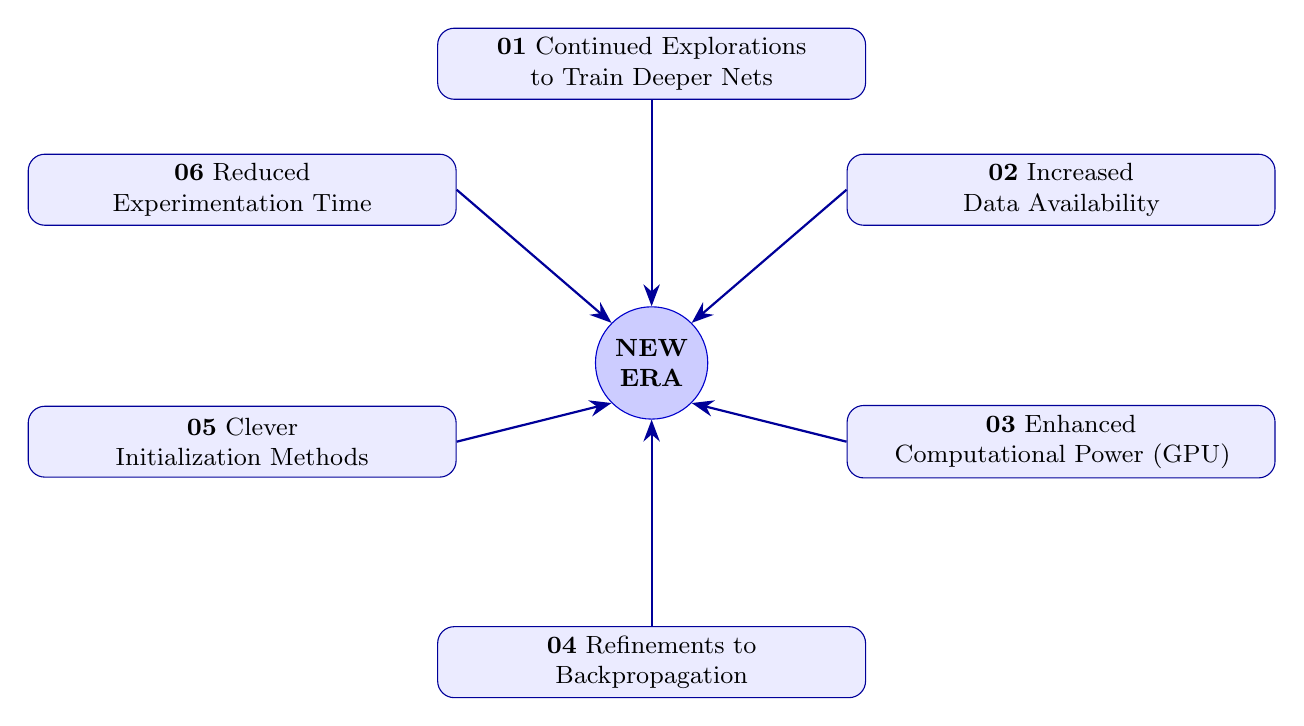
\begin{tikzpicture}[
  factor/.style={
    rectangle, rounded corners=6pt, draw=blue!60!black,
    fill=blue!8!white, text width=5.2cm, align=center,
    minimum height=0.9cm, font=\small
  },
  arrow/.style={-{Stealth[scale=1.2]}, thick, blue!60!black},
  label/.style={font=\bfseries\small, blue!80!black}
]

% Central node
\node[circle, draw=blue!80!black, fill=blue!20!white,
      minimum size=1.4cm, font=\bfseries\small, align=center]
  (center) at (0,0) {NEW\\ERA};

% Six factor nodes placed around the center
\node[factor] (f1) at (0, 3.8)
  {\textbf{01} Continued Explorations\\to Train Deeper Nets};
\node[factor] (f2) at (5.2, 2.2)
  {\textbf{02} Increased\\Data Availability};
\node[factor] (f3) at (5.2, -1.0)
  {\textbf{03} Enhanced\\Computational Power (GPU)};
\node[factor] (f4) at (0, -3.8)
  {\textbf{04} Refinements to\\Backpropagation};
\node[factor] (f5) at (-5.2, -1.0)
  {\textbf{05} Clever\\Initialization Methods};
\node[factor] (f6) at (-5.2, 2.2)
  {\textbf{06} Reduced\\Experimentation Time};

% Arrows pointing inward
\draw[arrow] (f1.south)  -- (center.north);
\draw[arrow] (f2.west)   -- (center.north east);
\draw[arrow] (f3.west)   -- (center.south east);
\draw[arrow] (f4.north)  -- (center.south);
\draw[arrow] (f5.east)   -- (center.south west);
\draw[arrow] (f6.east)   -- (center.north west);

\end{tikzpicture}
\caption{The six converging factors that enabled the deep learning
resurgence (slide V02, 00:22:00).  No single factor sufficed; all six
had to converge.}
\label{fig:six_factors}
\end{figure}

\begin{remark}
\label{rem:not_single_breakthrough}
Prof.\ Prasanna emphasised that the deep learning revolution was
\emph{not} the result of a single new algorithm.  The backpropagation
algorithm itself was not replaced; rather, external conditions
(data and compute) improved while targeted modifications to the
algorithm (weight initialisation and activation functions) addressed
the root cause of training failure.
\end{remark}

% -----------------------------------------------------------
% Table: Timeline of Neural Network Development
% -----------------------------------------------------------
\begin{table}[htbp]
\centering
\caption{Timeline of key milestones in neural network and deep learning
         history as discussed in the lecture.}
\label{tab:timeline}
\begin{tabular}{@{}lll@{}}
\toprule
\textbf{Period} & \textbf{Milestone} & \textbf{Significance} \\
\midrule
1950s--60s & Perceptron model proposed
           & First learnable neuron model \\
1986       & Backpropagation re-popularised
           & Enabled MLP training (2nd breakthrough) \\
Late 1980s & MLP with hidden layers demonstrated
           & Universal approximation capability shown \\
Early 1990s & ``AI hype'' era (neuro-fuzzy, etc.)
            & Performance only matched classical methods \\
Late 1990s & AI winter begins
           & Interest and funding declined \\
$\sim$2000 & Data digitisation explosion
           & Large datasets finally available \\
$\sim$2000 & GPU computing emerges
           & Parallel computation enables larger models \\
2006       & Hinton et al.\ greedy pre-training
           & First practical training of deep nets \\
2006--now  & Deep learning era
           & Continuous performance improvements \\
\bottomrule
\end{tabular}
\end{table}

% ===========================================================
\section{The Vanishing and Exploding Gradient Problem}
\label{sec:vgp}
% ===========================================================

\subsection{The Core Obstacle}
\label{subsec:core_obstacle}

The central problem that prevented deep network training for over a
decade is illustrated in \cref{fig:iceberg}, which reconstructs the
``iceberg diagram'' from lecture slide V03 (timestamp 00:37:35).

% -----------------------------------------------------------
% TikZ Diagram 2: Iceberg diagram (V03)
% -----------------------------------------------------------
\begin{figure}[htbp]
\centering
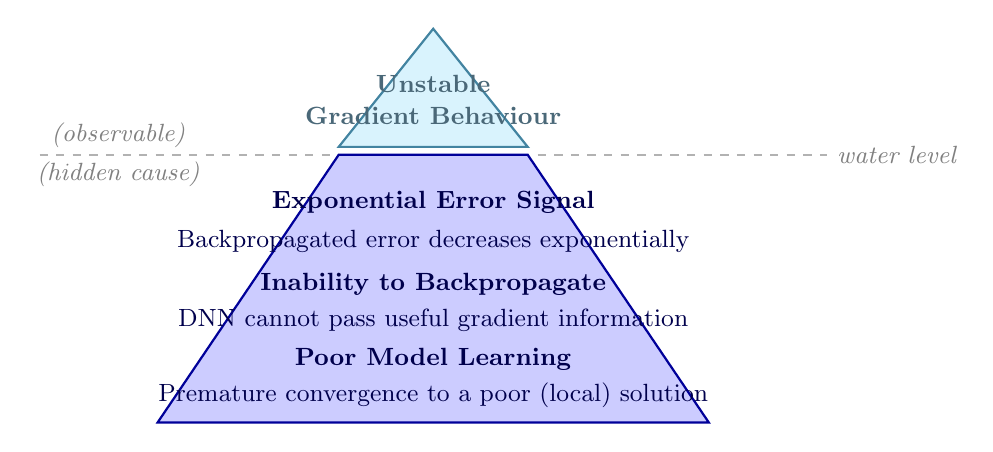
\begin{tikzpicture}[
  visible/.style={fill=cyan!15!white, draw=cyan!60!black, thick},
  hidden/.style={fill=blue!20!white, draw=blue!60!black, thick},
  label_vis/.style={font=\small\bfseries, text=cyan!40!black},
  label_hid/.style={font=\small, text=blue!30!black},
  waterline/.style={dashed, thick, gray!60}
]

% Iceberg tip (visible above water)
\fill[visible]
  (-1.2, 3.5) -- (0, 5.0) -- (1.2, 3.5) -- cycle;
\node[label_vis] at (0, 4.3) {Unstable};
\node[label_vis] at (0, 3.9) {Gradient Behaviour};

% Water line
\draw[waterline] (-5, 3.4) -- (5, 3.4)
  node[right, font=\small\itshape, gray] {water level};
\node[font=\small\itshape, gray] at (-4, 3.65) {(observable)};
\node[font=\small\itshape, gray] at (-4, 3.15) {(hidden cause)};

% Iceberg body (hidden below water)
\fill[hidden]
  (-1.2, 3.4) -- (-3.5, 0.0) -- (3.5, 0.0) -- (1.2, 3.4) -- cycle;

% Labels inside iceberg body
\node[label_hid, align=center] at (0, 2.8)
  {\textbf{Exponential Error Signal}};
\node[label_hid, align=center] at (0, 2.3)
  {Backpropagated error decreases exponentially};
\node[label_hid, align=center] at (0, 1.75)
  {\textbf{Inability to Backpropagate}};
\node[label_hid, align=center] at (0, 1.3)
  {DNN cannot pass useful gradient information};
\node[label_hid, align=center] at (0, 0.8)
  {\textbf{Poor Model Learning}};
\node[label_hid, align=center] at (0, 0.35)
  {Premature convergence to a poor (local) solution};

\end{tikzpicture}
\caption{Iceberg diagram of the VGP/EGP (slide V03, 00:37:35).  The
visible tip -- unstable training behaviour -- is the observable
symptom.  The real cause lies below the surface: exponential decay of
the backpropagated error signal.}
\label{fig:iceberg}
\end{figure}

\subsection{Mathematical Derivation}
\label{subsec:math_derivation}

Consider a network with layers indexed $l = 1, \ldots, L$.  At each
layer the pre-activation is $z^{(l)} = W^{(l)} a^{(l-1)}$ and the
activation is $a^{(l)} = f(z^{(l)})$ for some activation function~$f$.
The gradient of the loss with respect to the weight matrix of layer~1
is, by the chain rule (\cref{eq:backprop_chain}):

\begin{align}
  \frac{\partial \Loss}{\partial W^{(1)}}
  &= \frac{\partial \Loss}{\partial a^{(L)}}
     \cdot \prod_{l=2}^{L}
           \underbrace{f'(z^{(l)}) \cdot W^{(l)}}_{\text{one factor per layer}}
     \cdot x,
  \label{eq:chain_product}
\end{align}

where $x$ is the input.  For the logistic sigmoid, from
\cref{eq:sigmoid_deriv_bound}:

\begin{equation}
  f'(z^{(l)}) = \sigmoid'(z^{(l)}) \;\leq\; 0.25
  \quad \text{for all } z^{(l)}.
  \label{eq:sigmoid_max_deriv}
\end{equation}

If the weights are also initialised with magnitudes $|W^{(l)}| \leq 1$,
then each factor in the product of \cref{eq:chain_product} satisfies:

\begin{equation}
  \left| f'(z^{(l)}) \cdot W^{(l)} \right| \;\leq\; 0.25,
\end{equation}

so the product over $L-1$ layers is bounded by:

\begin{equation}
  \left| \prod_{l=2}^{L} f'(z^{(l)}) \cdot W^{(l)} \right|
  \;\leq\; (0.25)^{L-1}
  = 4^{-(L-1)}.
  \label{eq:exponential_decay}
\end{equation}

\Cref{eq:exponential_decay} shows that the gradient decays
exponentially in the depth $L$.  For a network with only five layers:
$4^{-4} = 1/256 \approx 0.004$ -- less than half a percent of the
original signal.

\begin{example}[title=Layer-by-Layer Gradient Decay]
\label{ex:gradient_decay}
Suppose every sigmoid derivative equals its maximum of $0.25$:
\begin{center}
\begin{tabular}{@{}lll@{}}
\toprule
\textbf{Layer} & \textbf{Gradient factor} & \textbf{Cumulative gradient} \\
\midrule
$L$ (output)   & 1.000 & 1.0000 \\
$L-1$          & $\times\;0.25$ & 0.2500 \\
$L-2$          & $\times\;0.25$ & 0.0625 \\
$L-3$          & $\times\;0.25$ & 0.0156 \\
$L-4$          & $\times\;0.25$ & 0.0039 \\
Layer 1 (input)& $\times\;0.25$ & $\approx 0.001$ \\
\bottomrule
\end{tabular}
\end{center}
By layer 1, the gradient is roughly 1000 times smaller than at the
output.  Weights in the early layers receive no meaningful update
signal.
\end{example}

\subsection{Numerical Walkthrough: Four-Layer Network}
\label{subsec:four_layer}

Dr.\ Saumya demonstrated the VGP with a minimal four-layer network
(one neuron per layer, sigmoid activations, all weights initialised to
$w = 0.5$, biases set to zero, single input $x_1 = 1$, target $y = 0$,
mean-squared loss).

\subsubsection{Forward Pass}
\label{subsubsec:forward}

The forward pass computes:

\begin{align}
  z^{(l)} &= w^{(l)} \cdot a^{(l-1)}, \qquad a^{(l)} = \sigmoid(z^{(l)}),
  \label{eq:forward_pass}
\end{align}

with $a^{(0)} = x_1 = 1$.  The numerical values are:

\begin{align}
  z_1 &= 0.5 \cdot 1 = 0.5, \quad a_1 = \sigmoid(0.5) \approx 0.6225, \notag\\
  z_2 &= 0.5 \cdot 0.6225 \approx 0.3113, \quad a_2 \approx 0.5771, \notag\\
  z_3 &= 0.5 \cdot 0.5771 \approx 0.2885, \quad a_3 \approx 0.5716, \notag\\
  z_4 &= 0.5 \cdot 0.5716 \approx 0.2858, \quad
        \hat{y} = a_4 \approx 0.5709. \label{eq:forward_values}
\end{align}

The loss (with the $\frac{1}{2}$ convenience factor):

\begin{equation}
  \Loss = \frac{1}{2}(\hat{y} - y)^2
        = \frac{1}{2}(0.5709 - 0)^2 \approx 0.1629.
  \label{eq:loss_value}
\end{equation}

\subsubsection{Backward Pass}
\label{subsubsec:backward}

Applying the chain rule from the output backwards:

\begin{align}
  \frac{\partial \Loss}{\partial \hat{y}}
  &= \hat{y} - y = 0.5709, \label{eq:dl_dyhat}\\[6pt]
  \frac{\partial \Loss}{\partial w_4}
  &= \frac{\partial \Loss}{\partial a_4} \cdot \sigmoid'(z_4) \cdot a_3
   \approx 0.5709 \times 0.2450 \times 0.5716
   \approx 0.0799, \label{eq:grad_w4}\\[6pt]
  \frac{\partial \Loss}{\partial w_3}
  &= \frac{\partial \Loss}{\partial w_4\text{-path}} \cdot w_4 \cdot
     \sigmoid'(z_3) \cdot a_2 \approx 0.0300, \label{eq:grad_w3}\\[6pt]
  \frac{\partial \Loss}{\partial w_2}
  &\approx 0.0110, \label{eq:grad_w2}\\[6pt]
  \frac{\partial \Loss}{\partial w_1}
  &\approx 0.0040. \label{eq:grad_w1}
\end{align}

\begin{keyinsight}
The gradient at layer~4 is $\approx 0.0799$.  By the time it reaches
layer~1, it has shrunk to $\approx 0.004$ -- \textbf{about 30 times
smaller}.  With a typical learning rate of $\eta = 0.01$, the weight
update at layer~1 is roughly $\Delta w_1 \approx 4 \times 10^{-5}$,
which is virtually zero.  The early layers \emph{do not learn}.
\end{keyinsight}

% ===========================================================
\section{Detailed Analysis of Sigmoid Saturation}
\label{sec:sigmoid}
% ===========================================================

\subsection{Why Sigmoid Saturates}
\label{subsec:sigmoid_saturation}

The logistic sigmoid function and its derivative are:

\begin{align}
  \sigmoid(z) &= \frac{1}{1 + e^{-z}}, \label{eq:sigmoid_def}\\[6pt]
  \sigmoid'(z) &= \sigmoid(z)\bigl(1 - \sigmoid(z)\bigr). \label{eq:sigmoid_prime}
\end{align}

For large $|z|$, $\sigmoid(z) \to 1$ or $\sigmoid(z) \to 0$.  In
either limit $\sigmoid'(z) \to 0$ because:

\begin{itemize}
  \item If $z \gg 0$: $\sigmoid(z) \approx 1$, so $\sigmoid'(z) \approx 1 \cdot (1-1) = 0$.
  \item If $z \ll 0$: $\sigmoid(z) \approx 0$, so $\sigmoid'(z) \approx 0 \cdot (1-0) = 0$.
\end{itemize}

The derivative is non-zero only in a narrow bell-shaped region around
$z = 0$, with maximum value $0.25$ attained at $z = 0$.  In deep
networks, the pre-activations $z^{(l)}$ frequently escape this narrow
range, driving the sigmoid into its flat regions and killing the
gradient.

\begin{remark}
\label{rem:tanh}
The hyperbolic tangent $\tanh(z) = 2\sigmoid(2z) - 1$ has the same
qualitative saturation behaviour.  Its derivative is bounded by~1
(at $z=0$) and also decays to zero for large $|z|$, so it does not
fundamentally solve the VGP.
\end{remark}

\subsection{Propagation Through Nested Sigmoids}
\label{subsec:nested_sigmoid}

In a deep sigmoid network, successive activations become increasingly
similar (saturate towards $0.5$ for zero-mean inputs).  As shown in
the forward-pass values of \cref{eq:forward_values}, the outputs
$a_1 \approx 0.622$, $a_2 \approx 0.577$, $a_3 \approx 0.572$,
$a_4 \approx 0.571$ differ by less and less -- the network enters the
flat region of the sigmoid, making the derivative contributions
near-zero.  This is the regime where the VGP is most severe.

\begin{warningbox}
In a deep network with sigmoid activations, even without extremely large
or small weights, the \emph{forward activations themselves saturate}.
This is because each sigmoid of a sigmoid of a sigmoid converges to a
fixed point.  The saturation is self-reinforcing: a saturated forward
activation produces a near-zero derivative in the backward pass,
which in turn prevents the early-layer weights from learning the
representations needed to un-saturate those activations.
\end{warningbox}

% -----------------------------------------------------------
% Algorithm: Backpropagation showing gradient decay
% -----------------------------------------------------------
\begin{algorithm}[htbp]
\caption{Backpropagation in a Deep Sigmoid Network (gradient trace)}
\label{alg:backprop_trace}
\SetAlgoLined
\KwIn{Network with $L$ sigmoid layers, weights $\{w^{(l)}\}$,
      input $x$, target $y$}
\KwOut{Gradients $\{\partial\Loss/\partial w^{(l)}\}$,
       showing exponential decay towards layer~1}

\tcp{--- Forward pass ---}
$a^{(0)} \leftarrow x$\;
\For{$l = 1$ \KwTo $L$}{
  $z^{(l)} \leftarrow W^{(l)} a^{(l-1)} + b^{(l)}$\;
  $a^{(l)} \leftarrow \sigmoid(z^{(l)})$\;
}
$\hat{y} \leftarrow a^{(L)}$\;
$\Loss \leftarrow \frac{1}{2}(\hat{y} - y)^2$\;

\tcp{--- Backward pass ---}
$\delta^{(L)} \leftarrow \hat{y} - y$ \tcp*{output gradient}
\For{$l = L$ \KwTo $1$}{
  $\displaystyle
  g^{(l)} \leftarrow \frac{\partial\Loss}{\partial w^{(l)}}
         = \delta^{(l)} \cdot \sigmoid'(z^{(l)}) \cdot a^{(l-1)}$\;
  \tcp{Propagate: each step multiplies by $\sigmoid'(\cdot) \leq 0.25$}
  $\delta^{(l-1)} \leftarrow \delta^{(l)} \cdot \sigmoid'(z^{(l)}) \cdot w^{(l)}$\;
  \texttt{// Note: } $|\delta^{(l-1)}| \leq 0.25 \cdot |\delta^{(l)}|$
  \texttt{ -- exponential decay!}\;
}
\Return $\{g^{(l)}\}_{l=1}^{L}$\;
\end{algorithm}

\subsection{Gradient Magnitude Table}
\label{subsec:gradient_table}

\Cref{tab:gradient_magnitudes} summarises the gradient magnitudes at
each layer in the four-layer demonstration.

\begin{table}[htbp]
\centering
\caption{Gradient magnitudes during backpropagation in the four-layer
         sigmoid network (from the lecture demonstration).  The gradient
         at layer~1 is approximately 30$\times$ smaller than at
         layer~4.}
\label{tab:gradient_magnitudes}
\begin{tabular}{@{}cccc@{}}
\toprule
\textbf{Layer} & \textbf{Activation $a^{(l)}$}
               & \textbf{Sigmoid derivative $\sigmoid'(z^{(l)})$}
               & \textbf{$\|\partial\Loss/\partial w^{(l)}\|$} \\
\midrule
4 (output) & 0.5709 & 0.2450 & 0.0799 \\
3          & 0.5716 & 0.2449 & 0.0300 \\
2          & 0.5771 & 0.2444 & 0.0110 \\
1 (early)  & 0.6225 & 0.2350 & 0.0040 \\
\bottomrule
\end{tabular}
\end{table}

% ===========================================================
\section{Solutions to the Vanishing Gradient Problem}
\label{sec:solutions}
% ===========================================================

Once the root cause was understood, researchers developed a three-step
solution framework, illustrated in \cref{fig:three_step_solution}
(reconstructed from lecture slide V05, timestamp 00:47:00).

% -----------------------------------------------------------
% TikZ Diagram 3: Three-step solution (V05)
% -----------------------------------------------------------
\begin{figure}[htbp]
\centering
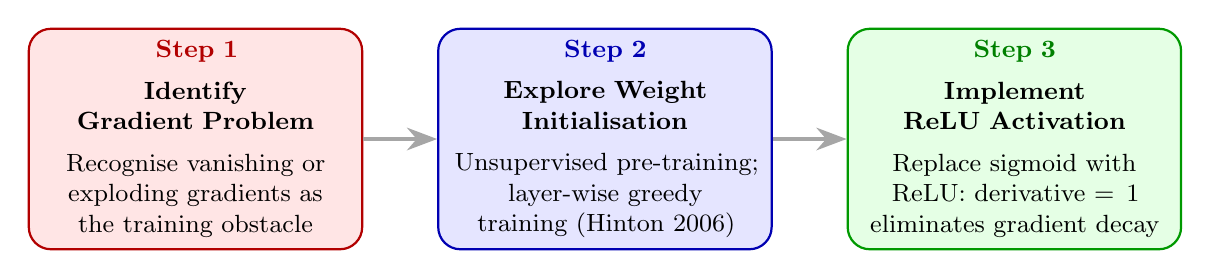
\begin{tikzpicture}[
  box/.style={
    rectangle, rounded corners=8pt, draw, thick,
    text width=4.0cm, align=center, minimum height=2.8cm,
    font=\small
  },
  step1/.style={box, fill=red!10!white,   draw=red!70!black},
  step2/.style={box, fill=blue!10!white,  draw=blue!70!black},
  step3/.style={box, fill=green!10!white, draw=green!60!black},
  arr/.style={-{Stealth[scale=1.3]}, very thick, gray!70}
]

\node[step1] (s1) at (0,0) {
  \textcolor{red!70!black}{\textbf{Step 1}}\\[4pt]
  \textbf{Identify}\\
  \textbf{Gradient Problem}\\[4pt]
  Recognise vanishing or\\exploding gradients as\\the training obstacle
};

\node[step2] (s2) at (5.2,0) {
  \textcolor{blue!70!black}{\textbf{Step 2}}\\[4pt]
  \textbf{Explore Weight}\\
  \textbf{Initialisation}\\[4pt]
  Unsupervised pre-training;\\layer-wise greedy\\training (Hinton 2006)
};

\node[step3] (s3) at (10.4,0) {
  \textcolor{green!50!black}{\textbf{Step 3}}\\[4pt]
  \textbf{Implement}\\
  \textbf{ReLU Activation}\\[4pt]
  Replace sigmoid with\\ReLU: derivative~$=1$\\eliminates gradient decay
};

\draw[arr] (s1.east) -- (s2.west);
\draw[arr] (s2.east) -- (s3.west);

\end{tikzpicture}
\caption{Three-step solution framework for VGP/EGP (slide V05,
         00:47:00).}
\label{fig:three_step_solution}
\end{figure}

\subsection{Solution 1 -- Weight Initialisation}
\label{subsec:weight_init}

The standard approach of \emph{random} initialisation starts the
network in a region of parameter space that may be far from anything
useful.  For deep networks, this is particularly harmful because even a
moderately poor initialisation places activations in the saturated
regions of sigmoid.

\subsubsection{Hinton's Greedy Layer-Wise Pre-Training (2006)}
\label{subsubsec:greedy_pretrain}

The breakthrough method proposed by Hinton, Osindero, and Teh (2006)
used \emph{unsupervised greedy pre-training} in a layer-wise fashion:

\begin{enumerate}
  \item Train the first layer as a Restricted Boltzmann Machine (RBM)
        or a simple autoencoder: learn weights $W^{(1)}$ that
        reconstruct the input from the first hidden representation.
        Minimise reconstruction error:
        \begin{equation}
          \Loss_1 = \bigl\| x - \hat{x}^{(1)} \bigr\|^2.
          \label{eq:recon_loss_1}
        \end{equation}
  \item Freeze $W^{(1)}$.  Use the learned representation $h^{(1)}$
        as the new ``input'' and train the second layer similarly:
        \begin{equation}
          \Loss_2 = \bigl\| h^{(1)} - \hat{h}^{(1)} \bigr\|^2.
          \label{eq:recon_loss_2}
        \end{equation}
  \item Repeat layer by layer up to depth~$L$.
  \item Use the pre-trained weights as the \emph{initialisation} for
        supervised fine-tuning via standard backpropagation.
\end{enumerate}

\begin{keyinsight}
Greedy pre-training solves the VGP indirectly: because each layer's
weights are already initialised to encode meaningful features of the
data (rather than random noise), the forward activations do not
immediately saturate, and backpropagation can usefully propagate
gradients all the way to the first layer.
\end{keyinsight}

\subsubsection{Modern Initialisation Methods}
\label{subsubsec:modern_init}

After 2010, it was found that carefully chosen random initialisations
could also avoid saturation at the start of training.  The two most
widely used are:

\begin{itemize}
  \item \textbf{Xavier / Glorot initialisation} (Glorot \&\ Bengio 2010):
        \begin{equation}
          W^{(l)} \sim \mathcal{U}\!\left(
            -\sqrt{\frac{6}{n_{\mathrm{in}}+n_{\mathrm{out}}}},\;
            +\sqrt{\frac{6}{n_{\mathrm{in}}+n_{\mathrm{out}}}}
          \right),
          \label{eq:xavier_init}
        \end{equation}
        where $n_{\mathrm{in}}$ and $n_{\mathrm{out}}$ are the number
        of input and output neurons of layer~$l$.  Designed to keep
        activation variances approximately constant across layers for
        sigmoid and tanh networks.

  \item \textbf{He initialisation} (He et al.\ 2015):
        \begin{equation}
          W^{(l)} \sim \mathcal{N}\!\left(
            0,\; \frac{2}{n_{\mathrm{in}}}
          \right),
          \label{eq:he_init}
        \end{equation}
        designed for ReLU activations.

  \item \textbf{Batch Normalisation} (Ioffe \&\ Szegedy 2015):
        normalises layer inputs to have zero mean and unit variance
        during each mini-batch, re-centering activations into the
        non-saturating region of sigmoid/tanh.
\end{itemize}

\subsection{Solution 2 -- ReLU Activation Function}
\label{subsec:relu}

The second major solution is to replace the sigmoid activation with
the \emph{Rectified Linear Unit}:

\begin{equation}
  \relu(z) = \max(0, z),
  \label{eq:relu_def}
\end{equation}

whose derivative is:

\begin{equation}
  \relu'(z) =
  \begin{cases}
    1 & \text{if } z > 0, \\
    0 & \text{if } z \leq 0.
  \end{cases}
  \label{eq:relu_deriv}
\end{equation}

When $z > 0$, the gradient is exactly~1 and does not shrink through
any number of layers.  This means:

\begin{equation}
  \prod_{l=2}^{L} \relu'(z^{(l)}) \in \{0, 1\},
  \quad\text{no exponential decay for active neurons.}
  \label{eq:relu_product}
\end{equation}

\begin{example}[title=ReLU Gradient Does Not Vanish]
\label{ex:relu_gradient}
With ReLU activations (and all pre-activations $z^{(l)} > 0$), the
gradient chain is:
\begin{center}
\begin{tabular}{@{}lll@{}}
\toprule
\textbf{Layer} & \textbf{ReLU derivative} & \textbf{Cumulative gradient} \\
\midrule
$L$   & 1 & 1.0 \\
$L-1$ & 1 & 1.0 \\
$L-2$ & 1 & 1.0 \\
$L-3$ & 1 & 1.0 \\
Layer 1 & 1 & 1.0 \\
\bottomrule
\end{tabular}
\end{center}
The gradient magnitude is preserved all the way to the first layer.
Compare with the sigmoid case in \cref{ex:gradient_decay}.
\end{example}

\subsubsection{ReLU Non-Linearity and the Dead Neuron Problem}
\label{subsubsec:dead_neuron}

A student raised an important question during the lecture: \emph{``Why
is ReLU preferred over tanh for the vanishing gradient, even though
ReLU can cause dead neurons?''}

ReLU is indeed non-linear (the ``kink'' at $z = 0$ breaks linearity),
which is necessary for deep networks to model complex functions.  For
$z > 0$ it is linear, making it easy to optimise and very fast to
compute.

However, the \emph{dying ReLU} problem arises when a neuron's
pre-activation $z^{(l)} \leq 0$ for all training samples, causing its
gradient to be identically zero and its weights to never update.
Variants of ReLU were proposed to address this:

\begin{description}
  \item[Leaky ReLU:] $f(z) = \max(\alpha z, z)$ for small
        $\alpha > 0$ (e.g.\ $\alpha = 0.01$), allowing a small negative
        gradient for $z < 0$.
  \item[ELU (Exponential Linear Unit):] $f(z) = z$ for $z \geq 0$,
        $\alpha(e^z - 1)$ for $z < 0$.
  \item[GELU (Gaussian Error Linear Unit):] $f(z) = z \cdot
        \Phi(z)$, used in Transformers.
\end{description}

\subsubsection{Sigmoid vs.\ ReLU: Full Comparison}
\label{subsubsec:sig_relu_comparison}

\Cref{tab:sig_vs_relu} gives the full comparison as presented in the
lecture visual extraction.

\begin{table}[htbp]
\centering
\caption{Comparison of sigmoid and ReLU activation functions.}
\label{tab:sig_vs_relu}
\begin{tabular}{@{}lll@{}}
\toprule
\textbf{Property}
  & \textbf{Sigmoid $\sigma(x)$}
  & \textbf{ReLU $\max(0,x)$} \\
\midrule
Output range    & $(0,\,1)$   & $[0,\,+\infty)$ \\
Derivative range & $(0,\,0.25]$ & $\{0,\,1\}$ \\
Vanishing gradient & \textbf{Yes} -- saturates at extremes
                   & \textbf{No} -- constant~1 for $x>0$ \\
Computational cost & Expensive ($e^{-x}$) & Very fast ($\max$) \\
Dying neurons      & No & \textbf{Yes} (for $x \leq 0$) \\
Biological plausibility & Higher & Lower \\
Typical use case  & Output layer (binary classification)
                  & Hidden layers (default choice) \\
\bottomrule
\end{tabular}
\end{table}

% ===========================================================
\section{Addressing VGP/EGP: Integrated View}
\label{sec:integrated_view}
% ===========================================================

\subsection{Why Both Solutions are Needed}
\label{subsec:both_needed}

ReLU alone does not fully eliminate the VGP.  Dead neurons create
regions of zero gradient that are structurally similar to sigmoid
saturation.  Likewise, good initialisation alone does not help if the
activation function accumulates saturation as training progresses.

The combination of \emph{better initialisation} and \emph{ReLU
activations} together proved sufficient to train the deep networks of
the 2006--2012 era.  Subsequent advances -- batch normalisation,
residual connections, and attention mechanisms -- further generalised
these principles.

\subsection{Layer-Wise Training: Modular Construction Analogy}
\label{subsec:layerwise}

Prof.\ Prasanna used an instructive analogy: layer-wise pre-training
is like modular construction in civil engineering.  Each module (layer)
is first built and tested in isolation, then assembled into the
complete structure.  In neural network terms:

\begin{itemize}
  \item Train (input $\to$ layer 1 $\to$ reconstruction of input).
  \item Freeze layer 1.  Train (layer 1 output $\to$ layer 2 $\to$
        reconstruction of layer 1 output).
  \item Repeat until all layers are pre-trained.
  \item Fine-tune the whole network end-to-end with backpropagation,
        using the pre-trained weights as a starting point.
\end{itemize}

The key insight is that the gradient only needs to travel through
\emph{one or two layers} during pre-training, so it never has a chance
to vanish.

\begin{keyinsight}
The backpropagation algorithm itself was \emph{not} discarded in the
deep learning revolution.  The community diagnosed exactly what was
going wrong (vanishing gradients due to sigmoid saturation and poor
initialisation) and applied targeted fixes.  The core algorithm
remained intact.
\end{keyinsight}

\subsection{Modern Perspective}
\label{subsec:modern_perspective}

Today, the dominant solution stack for avoiding VGP/EGP in practice is:

\begin{enumerate}
  \item \textbf{ReLU (or variant) activations} in all hidden layers.
  \item \textbf{He initialisation} for ReLU networks.
  \item \textbf{Batch Normalisation} after linear layers to maintain
        stable activation distributions during training.
  \item \textbf{Residual (skip) connections} (ResNet, 2015): allow
        the gradient to bypass entire blocks, providing ``shortcut''
        paths for the gradient that do not pass through activation
        functions.
\end{enumerate}

The greedy layer-wise pre-training of Hinton~(2006) is now largely of
historical interest, having been superseded by the above stack, but it
was the critical proof-of-concept that made the deep learning era
possible.

% ===========================================================
\section{Summary and Conclusions}
\label{sec:summary}
% ===========================================================

Session~8 covered the pivotal transition from shallow ANNs to deep
networks.  The following table summarises the key conceptual
contributions.

\begin{table}[htbp]
\centering
\caption{Session 8 -- Summary of key topics.}
\label{tab:summary}
\begin{tabular}{@{}p{4.2cm}p{9cm}@{}}
\toprule
\textbf{Topic} & \textbf{Key Message} \\
\midrule
Historical context
  & Deep networks were envisioned in the 1990s but could not be
    trained for $\sim$15 years due to the VGP. \\[4pt]
Six enabling factors
  & The deep learning revival was a convergence of data, compute,
    and algorithmic refinements -- not a single breakthrough. \\[4pt]
Vanishing gradient problem
  & Sigmoid derivatives $\leq 0.25$ cause gradients to shrink as
    $(0.25)^{L-1}$ exponentially with depth, starving early layers
    of training signal. \\[4pt]
Exploding gradient problem
  & Symmetric pathology; arises from floating-point overflow when
    derivatives compound in the forward direction. \\[4pt]
Weight initialisation
  & Hinton's greedy layer-wise unsupervised pre-training (2006)
    provided meaningful starting weights; modern alternatives
    include Xavier and He initialisation. \\[4pt]
ReLU activation
  & $\relu(z) = \max(0,z)$ has derivative~1 for $z>0$, preventing
    gradient decay; also computationally fast. \\[4pt]
Dead neuron problem
  & ReLU gradient is 0 for $z \leq 0$; addressed by Leaky ReLU,
    ELU, and other variants. \\
\bottomrule
\end{tabular}
\end{table}

\subsection{Looking Ahead}
\label{subsec:looking_ahead}

The next session continues the deep learning journey, examining
specific deep architectures (Convolutional Neural Networks, Recurrent
Neural Networks) and their training in detail.  The solutions
introduced here -- ReLU activations and principled weight
initialisation -- underpin all modern deep learning systems and will
appear repeatedly throughout the rest of the course.

\begin{keyinsight}
The deep learning era did not begin because computers got faster or
datasets grew larger in isolation.  It began because a small group of
researchers refused to abandon the field during its winter,
methodically diagnosed the root cause of training failure, and devised
solutions elegant enough to be adopted universally.
\end{keyinsight}

% ===========================================================
% APPENDIX
% ===========================================================
\appendix

\section{Mathematical Derivation: Sigmoid Derivative Upper Bound}
\label{app:sigmoid_bound}

\begin{theorem}
\label{thm:sigmoid_bound}
For the logistic sigmoid $\sigmoid(z) = \frac{1}{1+e^{-z}}$, the
derivative satisfies $\sigmoid'(z) \leq \frac{1}{4}$ for all
$z \in \mathbb{R}$.
\end{theorem}

\begin{proof}
From \cref{eq:sigmoid_prime}, $\sigmoid'(z) = \sigmoid(z)(1-\sigmoid(z))$.
Let $s = \sigmoid(z) \in (0,1)$.  We need to show $s(1-s) \leq 1/4$.
By AM-GM, $s(1-s) \leq \left(\frac{s + (1-s)}{2}\right)^2 = \frac{1}{4}$,
with equality iff $s = 1-s$, i.e.\ $s = 1/2$, i.e.\ $z = 0$.
\end{proof}

\begin{lemma}
\label{lem:product_decay}
For a sigmoid network with $L$ layers and weight magnitudes
$|W^{(l)}| \leq 1$, the gradient satisfies:
\begin{equation}
  \left|\frac{\partial\Loss}{\partial W^{(1)}}\right|
  \;\leq\;
  \left|\frac{\partial\Loss}{\partial a^{(L)}}\right|
  \cdot \left(\frac{1}{4}\right)^{L-1}.
  \label{eq:decay_bound}
\end{equation}
\end{lemma}

\begin{proof}
Follows directly from \cref{eq:chain_product,eq:sigmoid_max_deriv}
and the assumption $|W^{(l)}| \leq 1$.
\end{proof}

\section{ReLU Variants Reference}
\label{app:relu_variants}

\begin{table}[htbp]
\centering
\caption{Summary of ReLU variants mentioned in the lecture.}
\label{tab:relu_variants}
\begin{tabular}{@{}llll@{}}
\toprule
\textbf{Name} & \textbf{Definition} & \textbf{Derivative ($z<0$)}
              & \textbf{Notes} \\
\midrule
ReLU & $\max(0,z)$ & 0 & Standard; may cause dead neurons \\
Leaky ReLU & $\max(\alpha z, z)$ & $\alpha$ & $\alpha \approx 0.01$;
              prevents dead neurons \\
ELU & $z \geq 0$: $z$; $z<0$: $\alpha(e^z-1)$ & $\alpha e^z$ &
      Smooth; negative mean push \\
SELU & Self-normalising ELU & scaled & Auto-normalises activations \\
GELU & $z\,\Phi(z)$ & $\Phi(z) + z\phi(z)$ &
       Used in BERT, GPT \\
\bottomrule
\end{tabular}
\end{table}

\clearpage

%% ============================================================
%% Session 09: Mid-Course Quiz and Assessment Review
%% ============================================================
\part{Session 09: Mid-Course Quiz and Assessment Review}

%------------------------------------------------------------------

%==================================================================
% TITLE PAGE
%==================================================================
\begin{titlepage}
  \centering
  \vspace*{2cm}
  {\LARGE\bfseries Deep Learning -- Course Notes\par}
  \vspace{0.5cm}
  {\large IIIT Dharwad -- M.Tech / PhD Programme\par}
  \vspace{1.5cm}
  \rule{\linewidth}{0.4pt}\\[0.4cm]
  {\Huge\bfseries Session 09\par}
  \vspace{0.3cm}
  {\Large Mid-Course Quiz, Assessment Review,\\[4pt]
          and Foundations Consolidation\par}
  \rule{\linewidth}{0.4pt}\\[1.5cm]
  \begin{tabular}{ll}
    \textbf{Session number} & 09 \\[4pt]
    \textbf{Topic}          & Mid-course LMS quiz; post-quiz discussion \\[4pt]
    \textbf{Instructors}    & Prof.\ S R M Prasanna \& Dr.\ Sunil Saumya \\[4pt]
    \textbf{Teaching Asst.} & Vial (quiz coordinator) \\[4pt]
    \textbf{Slide deck}     & \texttt{05-PyTorchDL-NNmodule} \\[4pt]
    \textbf{Duration}       & $\approx 75$ minutes \\[4pt]
    \textbf{Date}           & Cohort 2, Academic Year 2025--26 \\
  \end{tabular}
  \vfill
  {\small These notes are reconstructed from the session transcript and\\
  visual extraction log (session09\_transcript.vtt).}
\end{titlepage}

%==================================================================
% TABLE OF CONTENTS
%==================================================================

\newpage

%==================================================================
\section{Introduction}
\label{sec:intro}
%==================================================================

Session~09 of the Deep Learning course at IIIT Dharwad served a dual
purpose.  The first and primary part consisted of a timed, LMS-based
mid-course quiz covering material from Sessions~01--08.  The second,
shorter part (roughly 15--20 minutes) was a live post-quiz review in
which Prof.\ Prasanna and the students discussed specific questions,
grading concerns, and the conceptual underpinning of incorrect or
disputed answers.

\medskip
\noindent
This document reconstructs the pedagogical content of that session.
It is structured as follows:
\begin{itemize}[leftmargin=1.5cm]
  \item \cref{sec:prereq} -- Prerequisites: a concise review of the
        topics on which the quiz was based.
  \item \cref{sec:quiz_logistics} -- Quiz logistics, format, and
        grading methodology.
  \item \cref{sec:quiz_topics} -- Topic-by-topic summary of the
        assessed concepts.
  \item \cref{sec:post_quiz_review} -- Post-quiz discussion: disputed
        questions, TensorFlow vs.\ PyTorch issue, and instructor
        clarifications.
  \item \cref{sec:vanishing_gradient} -- Deep-dive: vanishing gradient
        problem (the most-discussed quiz topic).
  \item \cref{sec:frameworks} -- PyTorch vs.\ TensorFlow: a comparative
        overview motivated by the quiz.
  \item \cref{sec:conclusion} -- Summary and outlook toward Sessions~10+.
\end{itemize}

\begin{keyinsight}
Session~09 is an \emph{assessment session}.  No new slides were presented
during the quiz period.  The post-quiz discussion, however, surfaced
several important conceptual clarifications about backpropagation,
gradient flow, and the relationship between PyTorch and TensorFlow --
all of which are examined in depth in this document.
\end{keyinsight}

%==================================================================
\section{Prerequisites and Background}
\label{sec:prereq}
%==================================================================

The quiz assessed cumulative knowledge from Sessions~01--08.  The
following subsections provide a concise review of each major building
block.

%------------------------------------------------------------------
\subsection{Perceptron and the Linear Threshold Unit}
\label{ssec:perceptron}
%------------------------------------------------------------------

A perceptron with $n$ inputs $x_1, \ldots, x_n$, weights
$w_1, \ldots, w_n$, and bias $b$ computes

\begin{equation}
  \hat{y} = \text{step}\!\left(\sum_{i=1}^{n} w_i x_i + b\right),
  \qquad
  \text{step}(z) = \begin{cases} 1 & z \geq 0 \\ 0 & z < 0 \end{cases}
  \label{eq:perceptron}
\end{equation}

\noindent
The \emph{perceptron learning rule} updates weights only when a
misclassification occurs:

\begin{equation}
  w_i \leftarrow w_i + \eta \,(y - \hat{y})\, x_i, \qquad
  b    \leftarrow b    + \eta \,(y - \hat{y})
  \label{eq:perceptron_update}
\end{equation}

\noindent
where $\eta > 0$ is the learning rate and $y \in \{0, 1\}$ is the
target.  The perceptron convergence theorem guarantees that, for any
linearly separable dataset, the algorithm terminates in a finite number
of steps.

\begin{definition}[Linear Separability]
\label{def:lin_sep}
A binary dataset $\{(\mathbf{x}_i, y_i)\}$ is \emph{linearly separable}
if there exists a hyperplane $\mathbf{w}^{\top}\mathbf{x} + b = 0$ such
that all samples with $y_i = 1$ lie on one side and all samples with
$y_i = 0$ lie on the other.
\end{definition}

A canonical non-linearly separable problem is XOR:

\begin{equation}
  \text{XOR}(0,0)=0,\quad
  \text{XOR}(0,1)=1,\quad
  \text{XOR}(1,0)=1,\quad
  \text{XOR}(1,1)=0.
  \label{eq:xor}
\end{equation}

\noindent
A single perceptron cannot solve XOR; a two-layer network (MLP) can.

%------------------------------------------------------------------
\subsection{Multi-Layer Perceptron and Forward Pass}
\label{ssec:mlp}
%------------------------------------------------------------------

An MLP with one hidden layer computes:
\begin{align}
  \mathbf{z}^{(1)} &= W^{(1)}\mathbf{x} + \mathbf{b}^{(1)},
    \label{eq:z1} \\
  \mathbf{a}^{(1)} &= f\!\left(\mathbf{z}^{(1)}\right),
    \label{eq:a1} \\
  \mathbf{z}^{(2)} &= W^{(2)}\mathbf{a}^{(1)} + \mathbf{b}^{(2)},
    \label{eq:z2} \\
  \hat{\mathbf{y}} &= g\!\left(\mathbf{z}^{(2)}\right),
    \label{eq:yhat}
\end{align}
where $f$ is a hidden-layer activation function and $g$ is an output
activation (e.g., softmax for classification or identity for regression).

\begin{remark}
\label{rem:matrix_order}
The convention adopted in PyTorch for a \emph{fully-connected} layer is
$\mathbf{z} = W\mathbf{x} + \mathbf{b}$, i.e., the weight matrix
multiplies the input vector from the \emph{left}.  In the post-quiz
review Prof.\ Prasanna noted that a TensorFlow snippet which placed the
input on the left ($\mathtt{tf.matmul}(X, W) + b$) confused several
students because the convention differs from the class exercises.
\end{remark}

%------------------------------------------------------------------
\subsection{Activation Functions}
\label{ssec:activations}
%------------------------------------------------------------------

\cref{tab:activations} summarises the activation functions covered in
Sessions~05--06.

\begin{table}[htbp]
  \centering
  \caption{Activation functions covered in Sessions~05--06.}
  \label{tab:activations}
  \begin{tabular}{lll}
    \toprule
    \textbf{Function} & \textbf{Formula} & \textbf{Range} \\
    \midrule
    Sigmoid   & $\sigma(z)=\dfrac{1}{1+e^{-z}}$            & $(0,1)$ \\[6pt]
    Tanh      & $\tanh(z)=\dfrac{e^z-e^{-z}}{e^z+e^{-z}}$ & $(-1,1)$ \\[6pt]
    ReLU      & $\max(0,z)$                                 & $[0,\infty)$ \\[4pt]
    Leaky ReLU & $\max(\alpha z,\,z),\;\alpha\ll 1$         & $(-\infty,\infty)$ \\[4pt]
    Step      & $\mathbf{1}[z \geq 0]$                      & $\{0,1\}$ \\
    \bottomrule
  \end{tabular}
\end{table}

%------------------------------------------------------------------
\subsection{Loss Functions}
\label{ssec:loss}
%------------------------------------------------------------------

For regression the Mean Squared Error (MSE) loss over $N$ samples is

\begin{equation}
  \loss_{\text{MSE}} = \frac{1}{N}\sum_{i=1}^{N}\bigl(y_i - \hat{y}_i\bigr)^2.
  \label{eq:mse}
\end{equation}

\noindent
For binary classification with the sigmoid output unit:

\begin{equation}
  \loss_{\text{BCE}} = -\frac{1}{N}\sum_{i=1}^{N}
    \Bigl[y_i \log\hat{y}_i + (1-y_i)\log(1-\hat{y}_i)\Bigr].
  \label{eq:bce}
\end{equation}

%------------------------------------------------------------------
\subsection{Backpropagation and the Chain Rule}
\label{ssec:backprop}
%------------------------------------------------------------------

Backpropagation computes $\partial \loss / \partial W^{(\ell)}$ for
each layer $\ell$ using the chain rule:

\begin{equation}
  \frac{\partial \loss}{\partial W^{(\ell)}}
  = \frac{\partial \loss}{\partial \mathbf{z}^{(\ell)}}
    \cdot
    \frac{\partial \mathbf{z}^{(\ell)}}{\partial W^{(\ell)}}.
  \label{eq:chain}
\end{equation}

\noindent
Defining the \emph{error signal} (delta) at layer $\ell$ as
$\boldsymbol{\delta}^{(\ell)} = \partial \loss / \partial
\mathbf{z}^{(\ell)}$, the backward recurrence is

\begin{align}
  \boldsymbol{\delta}^{(L)} &= \nabla_{\hat{\mathbf{y}}}\loss
    \odot g'\!\left(\mathbf{z}^{(L)}\right), \label{eq:delta_L} \\
  \boldsymbol{\delta}^{(\ell)} &=
    \left({W^{(\ell+1)}}^{\!\top}\boldsymbol{\delta}^{(\ell+1)}\right)
    \odot f'\!\left(\mathbf{z}^{(\ell)}\right), \label{eq:delta_l} \\
  \frac{\partial\loss}{\partial W^{(\ell)}} &=
    \boldsymbol{\delta}^{(\ell)}\,{\mathbf{a}^{(\ell-1)}}^{\!\top}, \label{eq:dL_dW}
\end{align}

\noindent
where $\odot$ denotes element-wise multiplication and $L$ is the number
of layers.

%==================================================================
\section{Quiz Logistics and Format}
\label{sec:quiz_logistics}
%==================================================================

%------------------------------------------------------------------
\subsection{Session Timeline}
\label{ssec:timeline}
%------------------------------------------------------------------

\cref{tab:timeline} gives the chronological structure of Session~09 as
reconstructed from the transcript.

\begin{table}[htbp]
  \centering
  \caption{Session~09 timeline.}
  \label{tab:timeline}
  \begin{tabularx}{\linewidth}{llX}
    \toprule
    \textbf{Timestamp} & \textbf{Phase} & \textbf{Activity} \\
    \midrule
    00:01:03 & Pre-quiz   & Students discussing exam logistics
                            (timing, links, LMS access) \\
    00:07:27 & Pre-quiz   & Session greeting; instructor joins; brief
                            mention of CNN as next topic \\
    00:08:30 & Pre-quiz   & Screen sharing started; instructions given \\
    00:22:18 & Quiz       & Quiz announced; LMS interface instructions \\
    00:23:19 & Quiz       & Camera-on requirement enforced \\
    00:24:17 & Quiz       & Quiz opens at 8:00 AM; students begin \\
    00:38:07 & Quiz       & Student raises question~8 (incomplete
                            $x_3 = 0.\!$\ldots value) \\
    00:48:29 & Post-quiz  & Quiz ends; class resumes \\
    00:49:51 & Post-quiz  & Student Q\&A on question~4 (duplicate
                            options A and C) \\
    00:57:59 & Post-quiz  & Prof.\ Prasanna joins; discusses TensorFlow
                            questions \\
    01:07:01 & Post-quiz  & Perceptron forward-pass question reviewed \\
    01:08:01 & Post-quiz  & Vanishing gradient question reviewed \\
    01:12:39 & Wrap-up    & Promise of 10--15 PyTorch practice questions
                            on LMS; session ends \\
    \bottomrule
  \end{tabularx}
\end{table}

%------------------------------------------------------------------
\subsection{Quiz Format}
\label{ssec:quiz_format}
%------------------------------------------------------------------

\begin{itemize}[leftmargin=1.5cm]
  \item \textbf{Platform:} IIIT Dharwad LMS (Moodle-based).
  \item \textbf{Number of questions:} 15 (multiple-choice).
  \item \textbf{Time limit:} 30 minutes from the moment of first access.
  \item \textbf{Access window:} 8:00 AM -- 9:30 AM (all students required
        to start at 8:00 AM to prevent sharing of questions).
  \item \textbf{Question order:} Randomised per student
        (``shuffled automatically'').
  \item \textbf{Camera:} Mandatory to keep the video feed on throughout.
  \item \textbf{Multiple correct answers:} Some questions had more than
        one correct option; students were advised to select the best
        available answer and grading would reflect the intent.
\end{itemize}

\begin{keyinsight}
  The instructor explicitly clarified that \emph{questions are shuffled
  automatically}, so the question numbers visible to different students
  differ.  This explains why students referring to ``question~8'' and
  ``question~13'' in the post-quiz review were discussing the same item
  from different perspectives.
\end{keyinsight}

%------------------------------------------------------------------
\subsection{Grading Policy}
\label{ssec:grading}
%------------------------------------------------------------------

\begin{itemize}[leftmargin=1.5cm]
  \item Automatic grading by the LMS at submission.
  \item Questions with TensorFlow code snippets (not covered in the
        course) were identified and \textbf{removed from grading}
        (approximately 2--3 questions).
  \item For questions in which multiple answers were debated,
        instructors reserved the right to review and update marks
        in the following session.
  \item The quiz score itself contributes to the continuous assessment
        component of the course.
\end{itemize}

\begin{warningbox}
  Three quiz questions used \texttt{tf.GradientTape} and
  \texttt{tf.matmul} syntax (TensorFlow API) rather than PyTorch.
  Because TensorFlow was \emph{never formally taught} in this course
  (PyTorch was used for all practicals), Prof.\ Prasanna confirmed that
  those questions would be \textbf{excluded from the final score}.
  Students are nevertheless encouraged to understand the conceptual
  equivalence: \texttt{tf.matmul(X,~W)~+~b} $\equiv$
  \texttt{torch.mm(X,~W)~+~b}, i.e., the maths is the same -- only
  the API differs.
\end{warningbox}

%==================================================================
\section{Quiz Topics: Concept-by-Concept Review}
\label{sec:quiz_topics}
%==================================================================

\cref{tab:quiz_coverage} maps each quiz topic area to the originating
session and the key concept being tested.

\begin{table}[htbp]
  \centering
  \caption{Mapping of quiz topics to course sessions.}
  \label{tab:quiz_coverage}
  \begin{tabularx}{\linewidth}{llX}
    \toprule
    \textbf{Topic Area} & \textbf{Sessions} & \textbf{Core Concept Tested} \\
    \midrule
    Perceptron learning rule    & 03--04 & Weight update, convergence guarantee \\
    Linear separability, XOR    & 04     & Why a single perceptron cannot solve XOR \\
    Backpropagation             & 05--07 & Chain rule, delta computation \\
    Activation functions        & 05--06 & Sigmoid, tanh, ReLU; saturation \\
    Forward pass (numerical)    & 05--06 & Manual computation of $z$ and $a$ \\
    Loss functions (MSE)        & 06     & MSE definition and gradient \\
    Chain rule / gradients      & 07     & Partial derivatives, composite functions \\
    Vanishing gradient          & 08     & Cause, effect, and depth dependence \\
    PyTorch tensor operations   & 02     & \texttt{torch.mm}, autograd \\
    \bottomrule
  \end{tabularx}
\end{table}

%------------------------------------------------------------------
\subsection{Sample Question: Perceptron Forward Pass}
\label{ssec:q_perceptron}
%------------------------------------------------------------------

One quiz question (question~8 in the original shuffled order seen by
some students) was a numerical perceptron forward pass.  The question
provided:

\begin{center}
  $x_1 = 1,\quad x_2 = 0,\quad x_3 = 0\;(\text{or } 0.0)$,
  \quad $w_1 = 0.5,\quad w_2 = -0.3,\quad w_3 = 0.2,\quad b = 0.1$.
\end{center}

Compute the output using the step activation function.

\begin{example}[Perceptron forward pass -- worked solution]
\begin{align}
  z &= w_1 x_1 + w_2 x_2 + w_3 x_3 + b \notag \\
    &= (0.5)(1) + (-0.3)(0) + (0.2)(0) + 0.1 \notag \\
    &= 0.5 + 0 + 0 + 0.1 = 0.6. \label{eq:perceptron_example}
\end{align}
Since $z = 0.6 \geq 0$, the step function outputs $\hat{y} = 1$.

\medskip
\noindent
\textit{Instructor note:} Whether $x_3 = 0$ or $x_3 = 0.0$ makes no
difference because $(0.2)(0) = 0$ in either case.  The final answer is
$\hat{y} = 1$.
\end{example}

\noindent
This underlines a common source of student confusion: floating-point
notation in quiz questions does not change the arithmetic.

%------------------------------------------------------------------
\subsection{Sample Question: Two-Layer MLP Forward Pass}
\label{ssec:q_mlp}
%------------------------------------------------------------------

Another question asked students to identify the correct code snippet
for a two-layer MLP forward pass and return the output tensor.

\begin{example}[Two-layer MLP forward pass -- PyTorch]
In PyTorch the canonical two-layer MLP forward pass is:
\begin{verbatim}
import torch
import torch.nn.functional as F

def forward(x, W1, b1, W2, b2):
    z1 = torch.mm(x, W1) + b1   # shape: (batch, hidden)
    a1 = F.relu(z1)
    z2 = torch.mm(a1, W2) + b2  # shape: (batch, output)
    return z2
\end{verbatim}
Note that in PyTorch's \texttt{nn.Linear} convention the weight matrix
$W$ has shape $(\text{out\_features}, \text{in\_features})$ and the
forward method computes $x W^{\top} + b$.  In the explicit
\texttt{torch.mm} form the user controls the order.
\end{example}

The equivalent TensorFlow snippet
\begin{verbatim}
y = tf.matmul(x, W) + b
\end{verbatim}
places the input $x$ first.  Several students were confused by this
reversal.  Prof.\ Prasanna confirmed: \textit{``To be frank, it
shouldn't be a $y$ here [on the left side of the equation] -- $y$
should be on the right side''}, referring to the question's labelling
inconsistency.

%==================================================================
\section{Post-Quiz Discussion: Key Clarifications}
\label{sec:post_quiz_review}
%==================================================================

The post-quiz discussion occupied roughly 15 minutes and was led jointly
by Prof.\ Prasanna and Dr.\ Saumya.  The following subsections
consolidate the substantive clarifications.

%------------------------------------------------------------------
\subsection{PyTorch vs.\ TensorFlow in the Quiz}
\label{ssec:tf_vs_pt}
%------------------------------------------------------------------

Students raised a valid concern: all class exercises used PyTorch, yet
several quiz questions used TensorFlow syntax.

\begin{keyinsight}
Prof.\ Prasanna's response captured the intended lesson:
\begin{quote}
  ``TensorFlow and PyTorch are just frameworks.  You have to see the
  \emph{internal operations}.  As soon as you see \texttt{matmul} -- that is
  matrix multiplication -- that much you have to understand.  Whether the
  API wraps it as \texttt{tf.matmul} or \texttt{torch.mm}, the
  \emph{maths is the same}.''
\end{quote}
\noindent
Despite this pedagogical point, the TensorFlow-specific questions were
removed from grading because TensorFlow was \emph{never formally introduced}
in the course.
\end{keyinsight}

\cref{tab:tf_pt_compare} provides a side-by-side comparison of the
most relevant operations.

\begin{table}[htbp]
  \centering
  \caption{PyTorch vs.\ TensorFlow API equivalence for common MLP operations.}
  \label{tab:tf_pt_compare}
  \begin{tabularx}{\linewidth}{lXX}
    \toprule
    \textbf{Operation} & \textbf{PyTorch} & \textbf{TensorFlow 2.x} \\
    \midrule
    Matrix multiply    & \texttt{torch.mm(A, B)} or \texttt{A @ B}
                       & \texttt{tf.matmul(A, B)} \\
    Element-wise add   & \texttt{A + B}             & \texttt{A + B} \\
    ReLU               & \texttt{F.relu(x)}         & \texttt{tf.nn.relu(x)} \\
    Sigmoid            & \texttt{torch.sigmoid(x)}  & \texttt{tf.sigmoid(x)} \\
    Gradient tape      & \texttt{loss.backward()}   & \texttt{tf.GradientTape()} \\
    Parameter update   & \texttt{optimizer.step()}  & \texttt{optimizer.apply\_gradients()} \\
    Zero gradients     & \texttt{optimizer.zero\_grad()} & N/A (tape-based) \\
    \bottomrule
  \end{tabularx}
\end{table}

%------------------------------------------------------------------
\subsection{Multiple-Correct-Answer Questions}
\label{ssec:multi_correct}
%------------------------------------------------------------------

Some questions had two equally valid answers (e.g., a lambda function
and a named function implementing the same operation).  The
instructor clarified:

\begin{quote}
  ``Some questions have both options also correct.  You can select which
  one is right for you.  We will check and evaluate.''
\end{quote}

\noindent
This is a known limitation of multiple-choice assessments for
programming tasks, where semantically equivalent code can be expressed
in multiple syntactic forms.

%------------------------------------------------------------------
\subsection{Vanishing Gradient -- Quiz Question Walkthrough}
\label{ssec:vanishing_quiz}
%------------------------------------------------------------------

The most substantive post-quiz discussion concerned a question about a
graph showing gradient magnitude (y-axis) versus layer number (x-axis).
The graph showed:
\begin{itemize}[leftmargin=1.5cm]
  \item Layers 1--6: steep gradient (high magnitude, declining).
  \item Layers 7--10: near-zero gradient (flat, almost zero).
\end{itemize}

The question asked: ``Which of the following is the most likely
consequence during training of this deep network?''

One option read: \textit{``Early layers will update significantly slower
than deeper layers because they receive smaller gradients.''}

\medskip
\noindent
A student argued this option should be correct, reasoning that in
backpropagation the gradient vanishes as it travels toward the input.
Prof.\ Prasanna's clarification was careful and important:

\begin{quote}
  ``See, based on the \emph{question graph}, gradients up to layer~6 are
  steep, so those layers will have a larger update.  The option says
  \emph{early layers} update slower, but in \emph{this particular graph}
  the early layers (1--6) still have a significant gradient.  It is the
  \emph{later} layers (7--10) where the gradient has already
  vanished.  The concept is the same; only the layer numbers shown in the
  figure are different from the classical presentation.  You must always
  answer relative to the information given in the question.''
\end{quote}

\begin{keyinsight}
This distinction is subtle but critical.  The classical vanishing
gradient problem states that \emph{gradients diminish as they propagate
backward from the output toward the input}, i.e., the earliest layers
receive the smallest gradients.  However, when a question provides a
\emph{specific graph} where the steep region covers layers~1--6 and the
flat region covers layers~7--10, the question refers to the \emph{later}
(deeper) layers receiving smaller gradients.  Students must read the
figure carefully rather than apply the textbook scenario blindly.
\end{keyinsight}

%==================================================================
\section{The Vanishing Gradient Problem: Deep Dive}
\label{sec:vanishing_gradient}
%==================================================================

Because the vanishing gradient was the most-discussed quiz topic, this
section provides a thorough treatment.

%------------------------------------------------------------------
\subsection{Mathematical Origin}
\label{ssec:vg_math}
%------------------------------------------------------------------

Consider a deep network with $L$ layers, each using a sigmoid
activation.  The gradient of the loss with respect to the weights in
layer~$\ell$ involves a product of terms:

\begin{equation}
  \frac{\partial \loss}{\partial W^{(\ell)}}
  \propto
  \prod_{k=\ell}^{L-1}
  \left[ {W^{(k+1)}}^{\!\top} \cdot \text{diag}\!\left(\sigma'\!\left(\mathbf{z}^{(k)}\right)\right) \right],
  \label{eq:vanishing_product}
\end{equation}

\noindent
where $\sigma'(z) = \sigma(z)\bigl(1-\sigma(z)\bigr) \leq 0.25$.

\begin{theorem}[Vanishing Gradient Bound]
\label{thm:vanishing}
If each weight matrix satisfies $\|W^{(k)}\|_2 \leq M$ and the
activation derivative satisfies $|f'(z)| \leq c < 1$, then for layer
$\ell$ in an $L$-layer network:
\begin{equation}
  \left\|\frac{\partial\loss}{\partial W^{(\ell)}}\right\|_2
  \;\leq\;
  K\,(Mc)^{L-\ell},
  \label{eq:vanishing_bound}
\end{equation}
where $K$ is a constant depending on the loss and the final-layer
gradient.  When $Mc < 1$ the bound decreases \emph{exponentially} with
depth $L - \ell$.
\end{theorem}

\begin{remark}
\label{rem:relu_fix}
The ReLU activation $f(z)=\max(0,z)$ has derivative $f'(z)=1$ for
$z>0$, which breaks the exponential decay for positive pre-activations.
This is why ReLU (and its variants such as Leaky ReLU and ELU) largely
replaced sigmoid/tanh in deep networks.
\end{remark}

%------------------------------------------------------------------
\subsection{TikZ Diagram: Gradient Flow in a Deep Network}
\label{ssec:tikz_gradient}
%------------------------------------------------------------------

\cref{fig:gradient_flow} illustrates how gradients of decreasing
magnitude flow backward through a deep sigmoid network.

\begin{figure}[htbp]
  \centering
  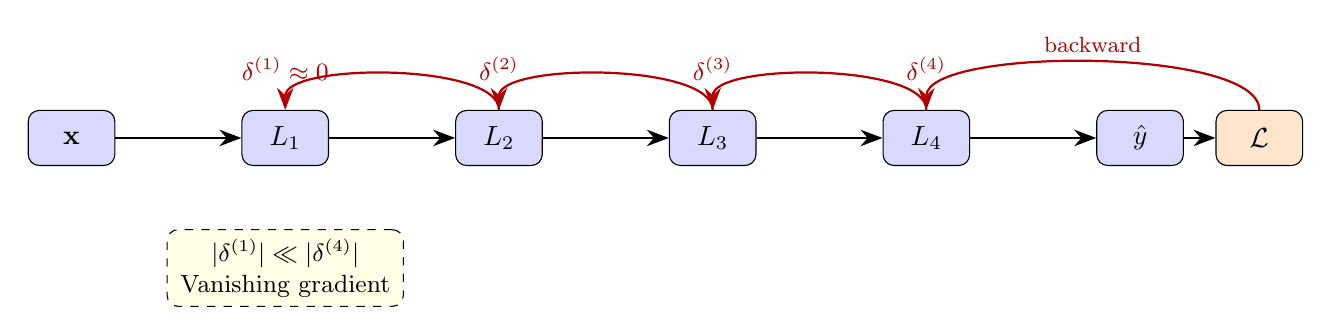
\begin{tikzpicture}[
      node distance=1.6cm,
      layer/.style={draw,rounded corners,minimum width=1.1cm,
                    minimum height=0.7cm,fill=blue!15},
      arrow/.style={-{Stealth[scale=1.2]},thick},
      gradarrow/.style={-{Stealth[scale=1.2]},thick,red!70!black},
    ]
    % Forward pass nodes
    \node[layer] (x)  {$\mathbf{x}$};
    \node[layer,right=of x]  (l1) {$L_1$};
    \node[layer,right=of l1] (l2) {$L_2$};
    \node[layer,right=of l2] (l3) {$L_3$};
    \node[layer,right=of l3] (l4) {$L_4$};
    \node[layer,right=of l4] (out){$\hat{y}$};
    \node[right=0.4cm of out,draw,fill=orange!20,rounded corners,
          minimum width=1.1cm,minimum height=0.7cm] (loss) {$\loss$};

    % Forward arrows
    \foreach \s/\t in {x/l1,l1/l2,l2/l3,l3/l4,l4/out,out/loss}
      \draw[arrow] (\s) -- (\t);

    % Gradient labels (decreasing magnitude)
    \node[above=0.25cm of l4,red!70!black,font=\small] (g4) {$\delta^{(4)}$};
    \node[above=0.25cm of l3,red!70!black,font=\small] (g3) {$\delta^{(3)}$};
    \node[above=0.25cm of l2,red!70!black,font=\small] (g2) {$\delta^{(2)}$};
    \node[above=0.25cm of l1,red!70!black,font=\small] (g1) {$\delta^{(1)} \approx 0$};

    % Backward arrows
    \draw[gradarrow] (loss.north) .. controls +(0,0.8) and +(0,0.8)
          .. node[above,font=\footnotesize]{backward} (l4.north);
    \draw[gradarrow] (l4.north) .. controls +(0,0.6) and +(0,0.6) .. (l3.north);
    \draw[gradarrow] (l3.north) .. controls +(0,0.6) and +(0,0.6) .. (l2.north);
    \draw[gradarrow] (l2.north) .. controls +(0,0.6) and +(0,0.6) .. (l1.north);

    % Magnitude annotation
    \node[below=0.8cm of l1,align=center,font=\small,
          draw,dashed,rounded corners,fill=yellow!10,
          minimum width=3cm] {
      $|\delta^{(1)}| \ll |\delta^{(4)}|$\\
      Vanishing gradient
    };

  \end{tikzpicture}
  \caption{Backward gradient flow in a 4-layer sigmoid network.  The
           gradient signal $\delta^{(\ell)}$ decreases exponentially
           as it travels from the output layer toward the input.}
  \label{fig:gradient_flow}
\end{figure}

%------------------------------------------------------------------
\subsection{TikZ Diagram: Sigmoid Saturation}
\label{ssec:tikz_sigmoid}
%------------------------------------------------------------------

\cref{fig:sigmoid_deriv} shows why the sigmoid derivative is bounded
above by $0.25$, the key mathematical cause of vanishing gradients.

\begin{figure}[htbp]
  \centering
  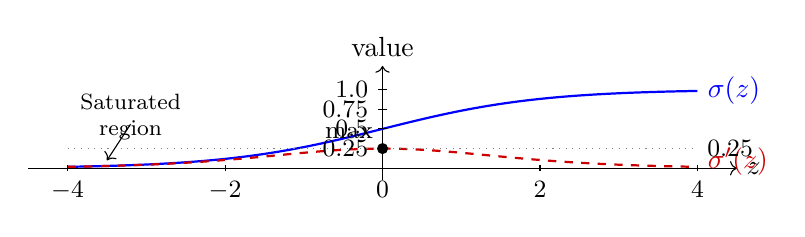
\begin{tikzpicture}[scale=1.0]
    % Axes
    \draw[->] (-4.5,0) -- (4.5,0) node[right] {$z$};
    \draw[->] (0,-0.15) -- (0,1.3) node[above] {value};

    % Sigmoid curve (piecewise linear approximation via control points)
    \draw[blue,thick,domain=-4:4,samples=100]
      plot (\x, {1/(1+exp(-\x))})
      node[right] {$\sigma(z)$};

    % Derivative curve
    \draw[red!80!black,thick,dashed,domain=-4:4,samples=100]
      plot (\x, {(1/(1+exp(-\x)))*(1-(1/(1+exp(-\x))))})
      node[right,yshift=2pt] {$\sigma'(z)$};

    % Max of derivative annotation
    \draw[gray,dotted] (-4,0.25) -- (4,0.25)
      node[right,font=\small,black] {$0.25$};
    \fill (0,0.25) circle (2pt) node[above left,font=\small] {max};

    % Saturation annotation
    \node[font=\footnotesize,align=center] at (-3.2,0.65)
      {Saturated\\region};
    \draw[->] (-3.2,0.56) -- (-3.5,0.1);

    % Ticks
    \foreach \x in {-4,-2,0,2,4}
      \draw (\x,0.04) -- (\x,-0.04) node[below,font=\small] {$\x$};
    \foreach \y in {0.25,0.5,0.75,1.0}
      \draw (0.06,\y) -- (-0.06,\y) node[left,font=\small] {$\y$};
  \end{tikzpicture}
  \caption{Sigmoid $\sigma(z)$ (solid blue) and its derivative
           $\sigma'(z)=\sigma(z)(1-\sigma(z))$ (dashed red).  The
           derivative is bounded above by $0.25$, and approaches zero
           in both saturated regions ($z \to \pm\infty$).}
  \label{fig:sigmoid_deriv}
\end{figure}

%------------------------------------------------------------------
\subsection{Mitigation Strategies}
\label{ssec:vg_mitigations}
%------------------------------------------------------------------

\begin{table}[htbp]
  \centering
  \caption{Strategies to mitigate the vanishing gradient problem.}
  \label{tab:vg_mitigations}
  \begin{tabularx}{\linewidth}{lX}
    \toprule
    \textbf{Strategy} & \textbf{Mechanism} \\
    \midrule
    ReLU activation      & Derivative is $1$ for $z > 0$; avoids
                           exponential decay \\
    Batch Normalisation  & Re-centres and re-scales activations per
                           mini-batch; reduces saturation \\
    Residual connections & Adds a skip connection $\mathbf{x} +
                           F(\mathbf{x})$; gradient can flow directly
                           through the skip path \\
    Weight initialisation & Xavier / He init ensures variance is
                            preserved across layers at the start of
                            training \\
    Gradient clipping    & Caps the gradient norm to prevent both
                           vanishing and exploding gradients \\
    LSTM / GRU gates     & Gating mechanism provides a \emph{constant
                           error carousel} for recurrent networks \\
    \bottomrule
  \end{tabularx}
\end{table}

%------------------------------------------------------------------
\subsection{Algorithm: Backpropagation with Gradient Monitoring}
\label{ssec:backprop_algo}
%------------------------------------------------------------------

\cref{alg:backprop} presents the backpropagation algorithm augmented
with a gradient-norm diagnostic step, which helps detect vanishing or
exploding gradients during training.

\begin{algorithm}[htbp]
  \DontPrintSemicolon
  \caption{Backpropagation with Gradient-Norm Monitoring}
  \label{alg:backprop}
  \KwIn{Network weights $\{W^{(\ell)}, \mathbf{b}^{(\ell)}\}_{\ell=1}^{L}$,
        input batch $(\mathbf{X}, \mathbf{Y})$,
        learning rate $\eta$, diagnostic flag \texttt{verbose}}
  \KwOut{Updated weights}
  \BlankLine
  \tcp{Forward pass}
  $\mathbf{a}^{(0)} \leftarrow \mathbf{X}$\;
  \For{$\ell = 1$ \KwTo $L$}{
    $\mathbf{z}^{(\ell)} \leftarrow W^{(\ell)}\mathbf{a}^{(\ell-1)} + \mathbf{b}^{(\ell)}$\;
    $\mathbf{a}^{(\ell)} \leftarrow f^{(\ell)}\!\left(\mathbf{z}^{(\ell)}\right)$\;
  }
  $\hat{\mathbf{Y}} \leftarrow \mathbf{a}^{(L)}$\;
  $\loss \leftarrow \frac{1}{N}\|\mathbf{Y} - \hat{\mathbf{Y}}\|^2$\;
  \BlankLine
  \tcp{Backward pass}
  $\boldsymbol{\delta}^{(L)} \leftarrow \frac{2}{N}(\hat{\mathbf{Y}} - \mathbf{Y}) \odot {f^{(L)}}'(\mathbf{z}^{(L)})$\;
  \For{$\ell = L-1$ \KwTo $1$}{
    $\boldsymbol{\delta}^{(\ell)} \leftarrow \left({W^{(\ell+1)}}^{\!\top}\boldsymbol{\delta}^{(\ell+1)}\right) \odot {f^{(\ell)}}'(\mathbf{z}^{(\ell)})$\;
    \If{\texttt{verbose}}{
      \textbf{print} $\ell$, $\|\boldsymbol{\delta}^{(\ell)}\|_2$\;
    }
  }
  \BlankLine
  \tcp{Weight update}
  \For{$\ell = 1$ \KwTo $L$}{
    $W^{(\ell)} \leftarrow W^{(\ell)} - \eta\,\boldsymbol{\delta}^{(\ell)}\,{\mathbf{a}^{(\ell-1)}}^{\!\top}$\;
    $\mathbf{b}^{(\ell)} \leftarrow \mathbf{b}^{(\ell)} - \eta\,\boldsymbol{\delta}^{(\ell)}\mathbf{1}$\;
  }
  \Return{$\{W^{(\ell)}, \mathbf{b}^{(\ell)}\}$}\;
\end{algorithm}

%==================================================================
\section{PyTorch vs.\ TensorFlow: A Framework Comparison}
\label{sec:frameworks}
%==================================================================

The quiz brought to light that students who had been taught exclusively
in PyTorch were unfamiliar with TensorFlow's eager-execution,
gradient-tape API.  This section provides the conceptual bridge.

%------------------------------------------------------------------
\subsection{Design Philosophy}
\label{ssec:design}
%------------------------------------------------------------------

\begin{keyinsight}
As Prof.\ Prasanna emphasised: \textit{``TensorFlow is maximum used for
production and PyTorch has been used for development and research
models.''  }Both frameworks implement the same mathematical operations.
The differences are primarily in API style and the execution model
(eager vs.\ graph-based compilation).
\end{keyinsight}

%------------------------------------------------------------------
\subsection{Gradient Computation: \texttt{autograd} vs.\ \texttt{GradientTape}}
\label{ssec:grad_compute}
%------------------------------------------------------------------

\paragraph{PyTorch autograd.}
\begin{verbatim}
import torch

x  = torch.tensor([[1.0, 0.0, 0.0]])
W1 = torch.randn(3, 4, requires_grad=True)
b1 = torch.zeros(4,  requires_grad=True)
W2 = torch.randn(4, 1, requires_grad=True)
b2 = torch.zeros(1,  requires_grad=True)

# Forward
z1 = x @ W1 + b1
a1 = torch.relu(z1)
z2 = a1 @ W2 + b2
loss = z2.mean()

# Backward
loss.backward()
print(W1.grad)   # dL/dW1
\end{verbatim}

\paragraph{TensorFlow 2 GradientTape.}
\begin{verbatim}
import tensorflow as tf

x  = tf.constant([[1.0, 0.0, 0.0]])
W1 = tf.Variable(tf.random.normal([3, 4]))
b1 = tf.Variable(tf.zeros([4]))
W2 = tf.Variable(tf.random.normal([4, 1]))
b2 = tf.Variable(tf.zeros([1]))

with tf.GradientTape() as tape:
    z1   = tf.matmul(x, W1) + b1
    a1   = tf.nn.relu(z1)
    z2   = tf.matmul(a1, W2) + b2
    loss = tf.reduce_mean(z2)

grads = tape.gradient(loss, [W1, b1, W2, b2])
print(grads[0])  # dL/dW1
\end{verbatim}

The key structural difference is that in PyTorch the computational
graph is built implicitly during the forward pass and
\texttt{.backward()} traverses it; in TensorFlow~2 the
\texttt{GradientTape} context manager \emph{explicitly records}
operations so that \texttt{tape.gradient} can replay them.  Conceptually
both implement \cref{eq:chain,eq:delta_L,eq:delta_l,eq:dL_dW}.

%------------------------------------------------------------------
\subsection{Architecture Diagram: PyTorch \texttt{nn.Module} MLP}
\label{ssec:tikz_nnmodule}
%------------------------------------------------------------------

\cref{fig:nnmodule} shows the component structure of a two-layer MLP
implemented with PyTorch's \texttt{nn.Module} API, which is the subject
of the slide deck referenced for Session~09
(\texttt{05-PyTorchDL-NNmodule}).

\begin{figure}[htbp]
  \centering
  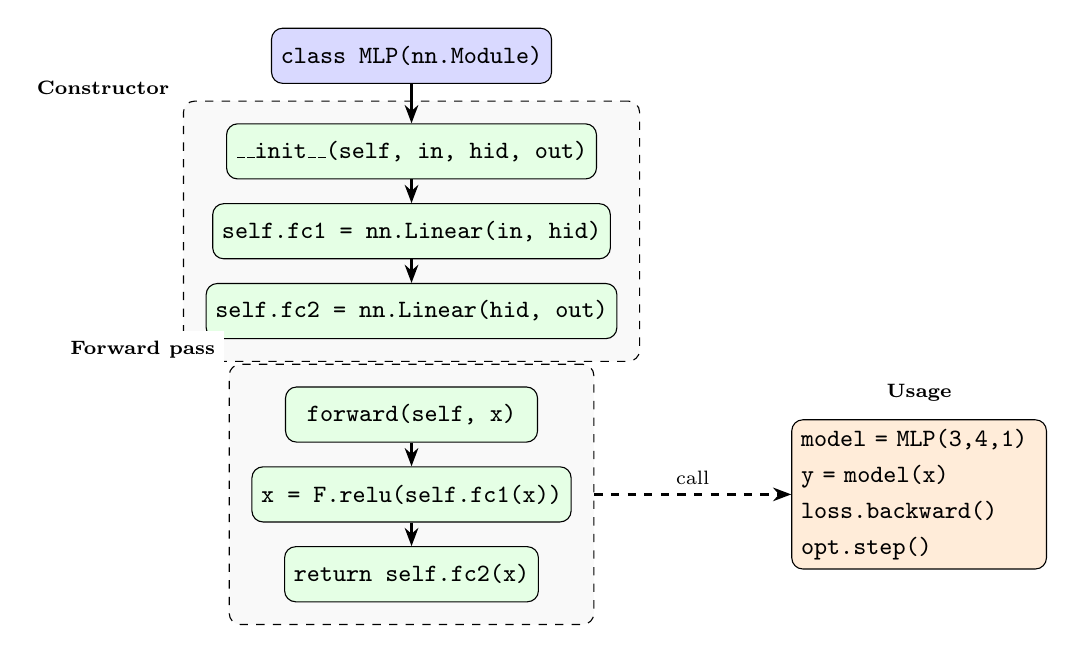
\begin{tikzpicture}[
      box/.style={draw,rounded corners,minimum width=3.2cm,
                  minimum height=0.7cm,fill=green!10,align=center,
                  font=\small},
      container/.style={draw,dashed,rounded corners,
                        fill=gray!5,inner sep=8pt},
      arrow/.style={-{Stealth},thick},
    ]

    % MLP class
    \node[box,fill=blue!15] (cls) {\texttt{class MLP(nn.Module)}};

    % __init__
    \node[box,below=0.5cm of cls] (init)
      {\texttt{\_\_init\_\_(self, in, hid, out)}};
    \node[box,below=0.3cm of init] (l1)
      {\texttt{self.fc1 = nn.Linear(in, hid)}};
    \node[box,below=0.3cm of l1]  (l2)
      {\texttt{self.fc2 = nn.Linear(hid, out)}};

    % forward
    \node[box,below=0.6cm of l2] (fwd)
      {\texttt{forward(self, x)}};
    \node[box,below=0.3cm of fwd] (r1)
      {\texttt{x = F.relu(self.fc1(x))}};
    \node[box,below=0.3cm of r1]  (r2)
      {\texttt{return self.fc2(x)}};

    % Container around __init__ block
    \begin{scope}[on background layer]
      \node[container,fit=(init)(l1)(l2)] (initbox) {};
      \node[container,fit=(fwd)(r1)(r2)]  (fwdbox)  {};
    \end{scope}
    \node[above left=-0.05cm and 0.05cm of initbox,
          font=\scriptsize,fill=white] {\textbf{Constructor}};
    \node[above left=-0.05cm and 0.05cm of fwdbox,
          font=\scriptsize,fill=white] {\textbf{Forward pass}};

    % Arrows
    \draw[arrow] (cls)  -- (init);
    \draw[arrow] (init) -- (l1);
    \draw[arrow] (l1)   -- (l2);
    \draw[arrow] (fwd)  -- (r1);
    \draw[arrow] (r1)   -- (r2);

    % Usage block
    \node[box,right=2.5cm of fwdbox,fill=orange!15,
          minimum width=3.2cm,align=left,
          text width=3cm] (usage) {%
      \texttt{model = MLP(3,4,1)}\\[2pt]
      \texttt{y = model(x)}\\[2pt]
      \texttt{loss.backward()}\\[2pt]
      \texttt{opt.step()}
    };
    \node[above=0.1cm of usage,font=\scriptsize\bfseries]
      {Usage};

    \draw[arrow,dashed] (fwdbox.east) -- (usage.west)
      node[midway,above,font=\scriptsize]{call};

  \end{tikzpicture}
  \caption{Structure of a two-layer MLP using PyTorch's
           \texttt{nn.Module} API, as covered in slide deck
           \texttt{05-PyTorchDL-NNmodule}.}
  \label{fig:nnmodule}
\end{figure}

%==================================================================
\section{Looking Ahead: CNN, RNN, LSTM, Transformer}
\label{sec:lookahead}
%==================================================================

At the conclusion of Session~09, Prof.\ Prasanna provided a brief
outlook on the remainder of the course.  His key message was:

\begin{quote}
  ``Once these fundamentals are in place -- one or two more classes on
  the \texttt{nn.Module} code -- we will enter into deep neural networks
  like CNN, RNN, LSTM, and even the transformer.  The fundamentals will
  not change much.  The architecture changes, but ultimately there will
  always be a backpropagation, and if you know how it works now, that is
  going to be the same for almost all the architectures you are going
  to study.''
\end{quote}

\cref{tab:architecture_comparison} shows how the core components of the
MLP extend to more complex architectures.

\begin{table}[htbp]
  \centering
  \caption{Extension of MLP fundamentals to advanced architectures.}
  \label{tab:architecture_comparison}
  \begin{tabularx}{\linewidth}{lXX}
    \toprule
    \textbf{Architecture} & \textbf{Key Addition over MLP}
                          & \textbf{Backprop variant} \\
    \midrule
    MLP           & Fully-connected layers only
                  & Standard backprop (\cref{alg:backprop}) \\
    CNN           & Convolutional + pooling layers; weight sharing
                  & Backprop through convolution \\
    RNN           & Recurrent hidden state; shared weights over time
                  & Backpropagation Through Time (BPTT) \\
    LSTM          & Gated memory cell; constant error carousel
                  & BPTT with vanishing-gradient mitigation \\
    Transformer   & Self-attention mechanism; no recurrence
                  & Backprop through attention weights \\
    \bottomrule
  \end{tabularx}
\end{table}

\begin{example}[Conceptual continuity from MLP to CNN]
In an MLP a hidden unit computes
$a_j = f\!\left(\sum_i w_{ji} x_i + b_j\right)$.
In a CNN a feature map at position $(r,c)$ computes
\[
  a_{rc} = f\!\!\left(\sum_{p}\sum_{q} k_{pq}\, x_{r+p,\,c+q} + b\right),
\]
where $k_{pq}$ is a \emph{shared} convolutional kernel.  The
backpropagation gradient with respect to $k_{pq}$ is simply
\[
  \frac{\partial\loss}{\partial k_{pq}}
  = \sum_{r}\sum_{c} \delta_{rc}\, x_{r+p,\,c+q},
\]
which is a cross-correlation of the error signal with the input patch --
entirely analogous to \cref{eq:dL_dW}.
\end{example}

%==================================================================
\section{Summary and Conclusion}
\label{sec:conclusion}
%==================================================================

Session~09 served as a pivotal checkpoint in the deep learning course.
The mid-course quiz assessed eight months of foundational material and
the subsequent discussion surfaced three important lessons.

\paragraph{Lesson 1 -- Read the figure, not only the concept.}
The vanishing gradient question demonstrated that exam answers must be
grounded in the \emph{specific scenario presented}, not just in the
canonical formulation.  A graph showing steeper gradients in early
layers and flat gradients in later layers inverts the classical picture;
the answer must reflect that inversion.

\paragraph{Lesson 2 -- Frameworks are wrappers, not new mathematics.}
The PyTorch/TensorFlow gap is syntactic, not mathematical.  Every
operation -- matrix multiply, gradient computation, parameter update --
maps directly to the same equation regardless of which framework
exposes it.  The ability to translate between API styles is a
professional skill, not a conceptual hurdle.

\paragraph{Lesson 3 -- Fundamentals are durable.}
As Prof.\ Prasanna emphasised, the chain rule, delta computation, and
gradient descent that underpin MLP training apply unchanged to CNN,
RNN, LSTM, and Transformer.  Investment in understanding these
fundamentals deeply pays compound interest throughout the remainder of
the course.

\medskip
\noindent
\textbf{Next session (Session~10)} resumes technical content with deep
feedforward networks and the PyTorch \texttt{nn.Module} framework in
detail.

\begin{keyinsight}
The core equations to remember from Sessions~01--09:
\begin{align}
  \text{Forward:}\quad
  \mathbf{z}^{(\ell)} &= W^{(\ell)}\mathbf{a}^{(\ell-1)} + \mathbf{b}^{(\ell)},
  \quad \mathbf{a}^{(\ell)} = f\!\left(\mathbf{z}^{(\ell)}\right), \notag \\
  \text{Backward:}\quad
  \boldsymbol{\delta}^{(\ell)} &=
    \left({W^{(\ell+1)}}^{\!\top}\boldsymbol{\delta}^{(\ell+1)}\right)
    \odot f'\!\left(\mathbf{z}^{(\ell)}\right), \notag \\
  \text{Update:}\quad
  W^{(\ell)} &\leftarrow W^{(\ell)}
    - \eta\,\boldsymbol{\delta}^{(\ell)}\,{\mathbf{a}^{(\ell-1)}}^{\!\top}. \notag
\end{align}
These three lines encode all of deep learning up to this point.
\end{keyinsight}

%------------------------------------------------------------------
\appendix
%------------------------------------------------------------------
\section{Quick Reference: Key Formulae}
\label{app:formulae}

\begin{align}
  &\text{Sigmoid:} & \sigma(z) &= \frac{1}{1+e^{-z}}, \quad
    \sigma'(z) = \sigma(z)(1-\sigma(z)) \leq 0.25, \label{eq:sig_ref}\\[4pt]
  &\text{Tanh:}    & \tanh'(z) &= 1 - \tanh^2(z) \leq 1, \label{eq:tanh_ref}\\[4pt]
  &\text{ReLU:}    & f'(z) &= \begin{cases}1 & z > 0 \\ 0 & z \leq 0\end{cases},
    \label{eq:relu_ref}\\[4pt]
  &\text{MSE:}     & \loss &= \frac{1}{N}\sum_i (y_i - \hat{y}_i)^2,
    \quad \frac{\partial\loss}{\partial\hat{y}_i} = \frac{-2}{N}(y_i - \hat{y}_i),
    \label{eq:mse_ref}\\[4pt]
  &\text{Perceptron update:} &
    w_i &\leftarrow w_i + \eta(y-\hat{y})x_i. \label{eq:perc_ref}
\end{align}

\section{PyTorch Snippet: Two-Layer MLP with Training Loop}
\label{app:pytorch}

The following complete snippet illustrates the PyTorch \texttt{nn.Module}
pattern and a basic training loop, synthesising the material assessed
in the quiz.

\begin{verbatim}
import torch
import torch.nn as nn
import torch.optim as optim

class TwoLayerMLP(nn.Module):
    def __init__(self, in_dim, hid_dim, out_dim):
        super().__init__()
        self.fc1 = nn.Linear(in_dim,  hid_dim)
        self.fc2 = nn.Linear(hid_dim, out_dim)

    def forward(self, x):
        x = torch.relu(self.fc1(x))
        return self.fc2(x)

# Instantiate
model = TwoLayerMLP(3, 8, 1)
criterion = nn.MSELoss()
optimizer = optim.SGD(model.parameters(), lr=0.01)

# Training loop
for epoch in range(100):
    optimizer.zero_grad()          # clear gradients
    y_hat = model(X_train)         # forward pass
    loss  = criterion(y_hat, y_train)
    loss.backward()                # backprop
    optimizer.step()               # update weights

    # Gradient norm monitoring (for vanishing gradient detection)
    for name, param in model.named_parameters():
        if param.grad is not None:
            print(f"{name}: grad norm = {param.grad.norm():.4f}")
\end{verbatim}

\clearpage

%% ============================================================
%% Session 10: Deep Feedforward Networks and Greedy Layer-wise Pre-training
%% ============================================================
\part{Session 10: Deep Feedforward Networks and Greedy Layer-wise Pre-training}

%% ===============================================================
%% TITLE PAGE
%% ===============================================================
\begin{titlepage}
  \centering
  \vspace*{1.5cm}
  {\LARGE\bfseries Deep Learning -- Session 10\par}
  \vspace{0.5cm}
  \rule{\linewidth}{1.5pt}\par
  \vspace{0.4cm}
  {\huge\bfseries Deep Feedforward Networks \&\\[0.3em]
   Greedy Layer-wise Pre-training\par}
  \vspace{0.4cm}
  \rule{\linewidth}{1.5pt}\par
  \vspace{1.2cm}
  {\large\itshape The 2006 Breakthrough: How Deep Networks Became Trainable\par}
  \vspace{1.5cm}
  \begin{tabular}{rl}
    \textbf{Session}      & 10 \\[4pt]
    \textbf{Date}         & December 21, 2025 \\[4pt]
    \textbf{Duration}     & 1 hour 40 minutes \\[4pt]
    \textbf{Instructors}  & Prof.\ S R M Prasanna \\
                          & Dr.\ Sunil Saumya \\[4pt]
    \textbf{Institution}  & Dept.\ of Data Science \& Artificial Intelligence \\
                          & Indian Institute of Information Technology Dharwad \\[4pt]
    \textbf{Slide Deck}   & \texttt{05-PyTorchDL-NNmodule} \\[4pt]
    \textbf{Video}        & \url{https://vimeo.com/1148825885} \\
  \end{tabular}
  \vspace{1.5cm}

  \begin{abstract}
    \noindent
    Session~10 covers the theoretical and empirical foundations of
    \emph{greedy layer-wise pre-training}, the pivotal technique introduced by
    Hinton et al.\ (2006) that made training deep networks feasible for the
    first time.  Starting from the observation that deep networks trained from
    random initialisation performed \emph{worse} than shallow networks due to
    vanishing/exploding gradients, the session explains how treating each hidden
    layer as a Restricted Boltzmann Machine (RBM) and pre-training it in
    isolation provides a principled weight initialisation.  The Bengio et al.\
    (2006, NIPS) supervised variant using auto-encoders is also presented.
    Landmark empirical results are reviewed: the deep generative model achieves
    1.25\% error on MNIST (vs.\ 1.4\% for SVM), and a DBN-DNN with 7 hidden
    layers achieves 17.1\% WER on the HUB500-SWB speech recognition benchmark
    (vs.\ 23.6\% for GMM-HMM).  The session concludes by contextualising why
    greedy pre-training is less necessary today given modern regularisation and
    optimisation advances (ReLU, batch normalisation, Adam), while noting its
    continued relevance for low-resource settings.
  \end{abstract}
\end{titlepage}

%% ===============================================================
%% TABLE OF CONTENTS
%% ===============================================================

\newpage

%% ===============================================================
\section{Introduction}
\label{sec:intro}
%% ===============================================================

The history of deep learning is punctuated by a small number of decisive
breakthroughs.  Session~10 focuses on the \textbf{2006 breakthrough} -- the
moment when the research community first demonstrated that deep neural networks
with many layers could be trained reliably and could outperform shallow
alternatives.

Prior to 2006, the neural network field had re-emerged from its first ``AI
winter'' thanks to the backpropagation algorithm, but a new ceiling had been
reached: adding more than two or three hidden layers consistently \emph{failed}
to improve performance, and often made things worse.  The culprits were the
\textbf{vanishing gradient} and \textbf{exploding gradient} problems discussed
in Session~9, which caused gradient-based optimisation starting from random
initialisation to become trapped in poor local minima.

\begin{keyinsight}[title=The Core Problem Before 2006]
  Deep neural networks (DNNs) possess enormous representational capacity,
  being capable of modelling highly non-linear and highly-varying functions.
  Yet in practice, training them from random initialisation using
  backpropagation produced results \emph{worse} than shallow networks with
  one or two hidden layers.  The bottleneck was the optimisation landscape,
  not the model architecture.
\end{keyinsight}

The solution, proposed simultaneously and independently by Hinton et al.\
\cite{hinton2006} and Bengio et al.\ \cite{bengio2006}, was a
\textbf{greedy layer-wise unsupervised pre-training} strategy.  By leveraging
techniques already used in the \emph{feedback} neural network literature
(specifically Restricted Boltzmann Machines) and applying them to
\emph{feedforward} networks, these groups demonstrated that deep networks could
be initialised in a region of weight space from which backpropagation could
refine them effectively.

This session covers:
\begin{enumerate}[leftmargin=*, label=\arabic*.]
  \item Why DNNs failed to train from random initialisation (\cref{sec:background}).
  \item The mechanics of unsupervised greedy layer-wise pre-training (\cref{sec:unsup}).
  \item The Bengio~(2006) supervised variant using auto-encoders (\cref{sec:sup}).
  \item Empirical results on MNIST (\cref{sec:mnist}) and large-vocabulary speech recognition (\cref{sec:asr}).
  \item The legacy and current relevance of pre-training (\cref{sec:legacy}).
\end{enumerate}

\newpage

%% ===============================================================
\section{Background and Prerequisites}
\label{sec:background}
%% ===============================================================

\subsection{Deep Feedforward Networks}

A \emph{deep feedforward network} (DFN), also called a \emph{multilayer
perceptron} (MLP) with many layers, is a directed acyclic graph of parametric
functions.  Given an input vector $\x \in \mathbb{R}^{d_0}$, the network
computes a sequence of hidden representations:

\begin{align}
  \h^{(1)} &= \sigma\!\left(\W^{(1)}\x + \mathbf{b}^{(1)}\right), \label{eq:h1} \\
  \h^{(\ell)} &= \sigma\!\left(\W^{(\ell)}\h^{(\ell-1)} + \mathbf{b}^{(\ell)}\right),
               \quad \ell = 2, \ldots, L, \label{eq:hl} \\
  \hat{y} &= \text{softmax}\!\left(\W^{(L+1)}\h^{(L)} + \mathbf{b}^{(L+1)}\right), \label{eq:yhat}
\end{align}

where $\sigma(\cdot)$ is a pointwise non-linear activation function
(e.g.\ sigmoid or tanh), $\W^{(\ell)}$ and $\mathbf{b}^{(\ell)}$ are the
weight matrix and bias vector for layer $\ell$, and $L$ is the total number
of hidden layers.

\begin{definition}[Depth of a Neural Network]
\label{def:depth}
  The \emph{depth} of a feedforward neural network is the number of
  \emph{hidden} layers $L$.  A network with $L = 1$ is called \emph{shallow};
  a network with $L \geq 2$ is typically called \emph{deep}.
\end{definition}

\subsection{The Vanishing Gradient Problem}

Training by backpropagation requires computing the gradient of the loss
$\loss$ with respect to the weights in every layer.  By the chain rule:

\begin{equation}
  \frac{\partial \loss}{\partial \W^{(1)}} =
  \frac{\partial \loss}{\partial \h^{(L)}} \cdot
  \prod_{\ell=2}^{L} \frac{\partial \h^{(\ell)}}{\partial \h^{(\ell-1)}} \cdot
  \frac{\partial \h^{(1)}}{\partial \W^{(1)}}.
  \label{eq:chain}
\end{equation}

Each Jacobian factor $\partial \h^{(\ell)}/\partial \h^{(\ell-1)}$ has entries
bounded by $\|\W^{(\ell)}\| \cdot \max|\sigma'(\cdot)|$.  For sigmoid
activations, $\max|\sigma'| = 0.25$, so the product in \cref{eq:chain}
\emph{shrinks exponentially} with depth, causing:

\begin{itemize}[leftmargin=*]
  \item \textbf{Vanishing gradients}: $\|\partial \loss / \partial \W^{(1)}\|
        \to 0$; early layers learn extremely slowly or not at all.
  \item \textbf{Exploding gradients}: When weight norms are large,
        the product diverges, causing numerical instability.
\end{itemize}

\begin{warningbox}
  Random weight initialisation places the network in a region of weight space
  where the gradients reaching the early layers are essentially zero.  The
  weights of the first few layers are therefore barely updated during training,
  producing representations no better than random projections of the input.
  This is the fundamental reason deep networks underperformed shallow ones
  before 2006.
\end{warningbox}

\subsection{Why One Hidden Layer ``Was Enough'' -- The Historical Debate}

Interestingly, before 2006, there was a compelling theoretical argument that
one hidden layer \emph{sufficed}:

\begin{theorem}[Universal Approximation, informal]
\label{thm:ua}
  A feedforward network with a single hidden layer of sufficiently many
  neurons can approximate any continuous function on a compact domain to
  arbitrary accuracy.
\end{theorem}

This theorem, combined with empirical results showing that networks with one
large hidden layer matched or exceeded multi-layer networks on tasks such as
speech recognition, led to a working consensus that depth added no benefit.
Support Vector Machines, with their kernel trick (effectively mapping data to
a very high-dimensional space for linear separation), appeared to confirm that
a single nonlinear expansion sufficed.

\begin{remark}
  The universal approximation theorem says \emph{existence} of a solution, not
  that gradient-based optimisation will \emph{find} it.  A single very wide
  layer may require exponentially more neurons than a deep network to represent
  certain functions efficiently.  Depth enables compositional representations
  that shallow networks cannot easily reproduce.
\end{remark}

\subsection{Three Converging Factors Behind the 2006 Breakthrough}

Prof.\ Prasanna emphasised in the lecture that the 2006 breakthrough was not
due to a single invention but to the convergence of three factors:

\begin{enumerate}[leftmargin=*, label=(\roman*)]
  \item \textbf{Large datasets}: The early 2000s saw the large-scale
        collection of labelled data (e.g.\ ImageNet, MNIST, Switchboard
        speech corpus), providing the fuel for data-hungry deep models.
  \item \textbf{GPU computing}: Graphics Processing Units offered
        massively parallel floating-point arithmetic at low cost, making
        large-scale matrix operations feasible.
  \item \textbf{Greedy layer-wise pre-training}: The algorithmic insight
        of Hinton et al.\ (2006) that each layer could be pre-trained
        independently using unsupervised reconstruction provided a principled
        initialisation that escaped poor local minima.
\end{enumerate}

\newpage

%% ===============================================================
\section{Unsupervised Greedy Layer-wise Pre-training}
\label{sec:unsup}
%% ===============================================================

\subsection{The Core Idea}

The term \emph{greedy layer-wise} describes a strategy that breaks an
otherwise intractable joint optimisation problem into a sequence of simpler
sub-problems, each solved independently.  The key observation is:

\begin{keyinsight}[title=Greediness in Pre-training]
  When training a given hidden layer, we \emph{ignore} the effect of all
  higher layers.  We are ``greedy'' in the sense that the sole objective
  for each layer is to best reconstruct its own input.  Since no target
  output is available, this is an \emph{unsupervised} procedure.
\end{keyinsight}

Concretely, consider a DFN with $L = 5$ hidden layers
$H_1, H_2, \ldots, H_5$ between the input $\x$ and the output $\hat{y}$.
Instead of training all weights jointly (which leads to vanishing gradients
at $H_1$), we train one layer at a time:

\begin{enumerate}[leftmargin=*, label=\textbf{Step \arabic*:}]
  \item \textbf{Pre-train $H_1$}: Treat the pair (input layer, $H_1$) as a
        two-layer \emph{feedback} (recurrent) network.  Apply input $\x$,
        propagate forward to $H_1$, then propagate \emph{back} to produce a
        reconstruction $\hat{\x}$.  Minimise the reconstruction error
        $\|\x - \hat{\x}\|^2$.  The resulting weight matrix $\W^{(1)}$
        captures the distribution of $\x$.
  \item \textbf{Pre-train $H_2$}: Pass all training inputs through the
        now-frozen $\W^{(1)}$ to obtain the activations of $H_1$.  Use
        these as the input to a new two-layer feedback network and pre-train
        $\W^{(2)}$ in the same way.
  \item \textbf{Repeat} for $H_3, H_4, H_5$ using the outputs of the
        previously trained layers as inputs.
  \item \textbf{Stack and fine-tune}: Assemble all pre-trained layers into the
        full deep network.  Attach a classification output layer with randomly
        initialised weights $\W^{(L+1)}$.  Fine-tune the entire network
        end-to-end using standard backpropagation (typically for only a few
        epochs, since the weights are already in a good region).
\end{enumerate}

\subsection{Mathematical Formulation of Pre-training a Single Layer}

For layer $\ell$, let the input be $\mathbf{v} \in \mathbb{R}^{d_{\ell-1}}$
(the output of the previous layer, or the raw input for $\ell = 1$).  The
reconstruction objective is:

\begin{equation}
  \min_{\W^{(\ell)}, \mathbf{b}^{(\ell)}}
  \; \mathbb{E}_{\mathbf{v}}\!\left[
    \left\| \mathbf{v} - \hat{\mathbf{v}} \right\|^2
  \right],
  \label{eq:recon}
\end{equation}

where the reconstructed input $\hat{\mathbf{v}}$ is obtained by:

\begin{align}
  \h &= \sigma\!\left(\W^{(\ell)}\mathbf{v} + \mathbf{b}^{(\ell)}\right),
       \label{eq:enc} \\
  \hat{\mathbf{v}} &= \sigma\!\left({\W^{(\ell)}}^{\!\top}\h + \tilde{\mathbf{b}}^{(\ell)}\right).
       \label{eq:dec}
\end{align}

Here ${\W^{(\ell)}}^{\!\top}$ is the transposed weight matrix (tied weights),
acting as the decoder.  Once the reconstruction error is minimised, $\W^{(\ell)}$
encodes a faithful representation of the input data distribution.

\begin{remark}
  The use of tied weights (decoder = encoder$^\top$) in \cref{eq:dec} is not
  mandatory.  In practice, the Hinton group used Restricted Boltzmann Machines
  (RBMs), which learn the weight matrix through contrastive divergence.  For
  the first (visible) layer they used a \emph{Gaussian} RBM (GRBM) to handle
  continuous-valued inputs.  The key distinction between an RBM-based approach
  and a simple auto-encoder is the probabilistic treatment of the hidden
  activations, but conceptually both achieve the same goal: learning a weight
  matrix that preserves the input statistics.
\end{remark}

\subsection{The Role of the Final (Output-Side) Weight Matrix}

A subtle but important point raised in the lecture is why $\W^{(L+1)}$
(the weights connecting the last hidden layer to the output) is \emph{not}
pre-trained and is instead randomly initialised:

\begin{keyinsight}[title=Why $\W^{(L+1)}$ is Randomly Initialised]
  The purpose of pre-training is to provide good generative representations of
  the input.  The output weight matrix $\W^{(L+1)}$ is a \emph{discriminative}
  layer: its job is to separate classes, not to reconstruct the input.
  Because the output layer is directly adjacent to the loss, its gradient is
  large and well-defined during fine-tuning.  There is no vanishing gradient
  problem for $\W^{(L+1)}$; backpropagation can learn it effectively from
  scratch.
\end{keyinsight}

\subsection{The GRBM $\rightarrow$ RBM $\rightarrow$ DBN $\rightarrow$ DBN-DNN Pipeline}

\cref{fig:dbn-pipeline} illustrates the four-step pipeline used by Hinton
et al.\ (2012) for acoustic modelling with DNNs.

\begin{figure}[ht]
\centering
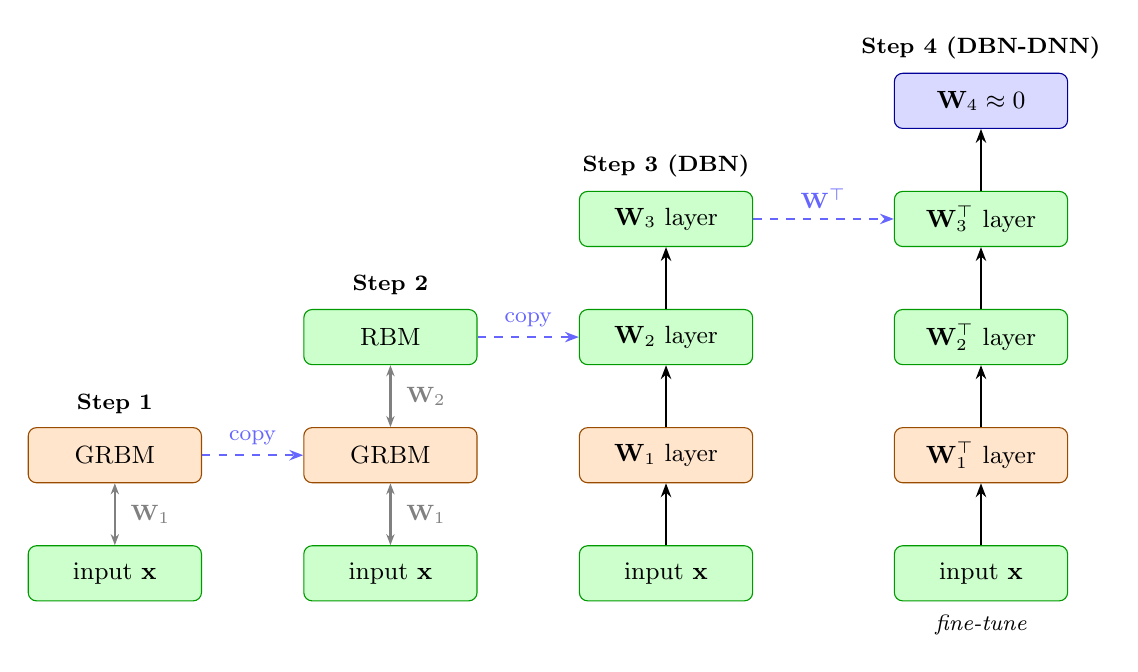
\begin{tikzpicture}[
  every node/.style={font=\small},
  layer/.style={draw, rounded corners=3pt, minimum width=2.2cm, minimum height=0.7cm,
                fill=green!20, draw=green!60!black},
  weight/.style={font=\footnotesize\itshape, midway, right=2pt},
  arr/.style={-{Stealth[length=5pt]}, thick},
  darr/.style={{Stealth[length=4pt]}-{Stealth[length=4pt]}, thick, gray},
  box/.style={draw=gray!70, dashed, rounded corners=5pt, inner sep=6pt}
]

%% Step 1: Train GRBM
\node[layer, fill=orange!20, draw=orange!60!black] (grbm) at (0,1.5) {GRBM};
\node[layer] (in1) at (0,0) {input $\mathbf{x}$};
\draw[darr] (in1.north) -- node[weight]{$\W_1$} (grbm.south);
\node[above=0.05cm of grbm, font=\footnotesize\bfseries] {Step 1};

%% Step 2: Stack RBMs
\node[layer] (rbm2) at (3.5,3.0) {RBM};
\node[layer, fill=orange!20, draw=orange!60!black] (grbm2) at (3.5,1.5) {GRBM};
\node[layer] (in2) at (3.5,0) {input $\mathbf{x}$};
\draw[darr] (in2.north) -- node[weight]{$\W_1$} (grbm2.south);
\draw[darr] (grbm2.north) -- node[weight]{$\W_2$} (rbm2.south);
\node[above=0.05cm of rbm2, font=\footnotesize\bfseries] {Step 2};
\draw[arr, dashed, blue!60] (grbm.east) -- node[above, font=\footnotesize]{copy} (grbm2.west);

%% Step 3: DBN
\node[layer] (w3) at (7,4.5) {$\W_3$ layer};
\node[layer] (w2) at (7,3.0) {$\W_2$ layer};
\node[layer, fill=orange!20, draw=orange!60!black] (w1) at (7,1.5) {$\W_1$ layer};
\node[layer] (in3) at (7,0) {input $\mathbf{x}$};
\draw[arr] (in3.north) -- (w1.south);
\draw[arr] (w1.north) -- (w2.south);
\draw[arr] (w2.north) -- (w3.south);
\node[above=0.05cm of w3, font=\footnotesize\bfseries] {Step 3 (DBN)};

%% Step 4: DBN-DNN fine-tune
\node[layer, fill=blue!15, draw=blue!60!black] (w4) at (11,6.0) {$\W_4 \approx 0$};
\node[layer] (w3t) at (11,4.5) {$\W_3^\top$ layer};
\node[layer] (w2t) at (11,3.0) {$\W_2^\top$ layer};
\node[layer, fill=orange!20, draw=orange!60!black] (w1t) at (11,1.5) {$\W_1^\top$ layer};
\node[layer] (in4) at (11,0) {input $\mathbf{x}$};
\draw[arr] (in4.north) -- (w1t.south);
\draw[arr] (w1t.north) -- (w2t.south);
\draw[arr] (w2t.north) -- (w3t.south);
\draw[arr] (w3t.north) -- (w4.south);
\node[above=0.05cm of w4, font=\footnotesize\bfseries] {Step 4 (DBN-DNN)};
\node[below=0.05cm of in4, font=\footnotesize\itshape] {fine-tune};

%% Arrows between steps
\draw[arr, dashed, blue!60] (rbm2.east) -- node[above, font=\footnotesize]{copy} (w2.west);
\draw[arr, dashed, blue!60] (w3.east) -- node[above, font=\footnotesize]{$\W^\top$} (w3t.west);

\end{tikzpicture}
\caption{The four-step greedy layer-wise pre-training pipeline for
acoustic modelling (Hinton et al., IEEE Signal Processing Magazine, 2012).
GRBM: Gaussian Restricted Boltzmann Machine (used for the visible layer with
continuous inputs); RBM: Restricted Boltzmann Machine for higher layers;
DBN: Deep Belief Network formed by stacking RBMs; DBN-DNN: the DBN weights
are used as initialisation for a discriminatively fine-tuned DNN.
$\W_4 \approx 0$ indicates the output layer is randomly (near-zero) initialised.}
\label{fig:dbn-pipeline}
\end{figure}

\subsection{Why the Term ``Greedy''?}

The term \emph{greedy} has a precise meaning here.  In combinatorial
optimisation, a greedy algorithm makes the locally optimal choice at each
step without considering the global impact.  In the context of layer-wise
pre-training:

\begin{itemize}[leftmargin=*]
  \item When training layer $\ell$, we do not consider layers $\ell+1, \ldots, L$.
  \item The optimisation objective for layer $\ell$ is purely local: minimise
        the reconstruction error of its own input.
  \item Interaction between layers is handled only during the final
        end-to-end fine-tuning phase.
\end{itemize}

This local, independent training sidesteps the vanishing gradient problem
entirely during the pre-training phase, since each sub-network has only two
layers and gradients flow freely.

\newpage

%% ===============================================================
\section{Supervised Greedy Layer-wise Pre-training (Bengio et al., 2006)}
\label{sec:sup}
%% ===============================================================

\subsection{Motivation: Adding Supervision to Pre-training}

Hinton et al.\ (2006) used purely \emph{unsupervised} pre-training -- no
class labels were used during the layer-by-layer initialisation phase.
Bengio et al.\ (2006), published at NIPS~2006, independently confirmed these
results and additionally proposed a \emph{supervised} variant, where each
layer is trained with access to target class information.

\subsection{Auto-encoders as the Supervised Pre-training Vehicle}

The mechanism for supervised pre-training is based on the
\textbf{auto-encoder} architecture.

\begin{definition}[Auto-encoder]
\label{def:autoencoder}
  An \emph{auto-encoder} is a feedforward neural network trained to reproduce
  its input at its output.  Given input $\x$, the network minimises:
  \begin{equation}
    \loss_{\text{AE}} = \|\x - f_{\text{dec}}(f_{\text{enc}}(\x))\|^2,
    \label{eq:ae-loss}
  \end{equation}
  where $f_{\text{enc}}$ is the \emph{encoder} (maps $\x$ to a latent
  representation $\mathbf{z}$) and $f_{\text{dec}}$ maps $\mathbf{z}$ back
  to the input space.  The target output is identical to the input: the
  network is forced to ``look at itself in the mirror.''
\end{definition}

\begin{example}[Auto-encoder for Pre-training Layer 1]
  Suppose the input dimension is 784 (a flattened $28 \times 28$ MNIST image)
  and the first hidden layer has 500 neurons.  For supervised pre-training:
  \begin{enumerate}
    \item Build a three-layer auto-encoder: $784 \to 500 \to 784$.
    \item Set the target output equal to the input.
    \item Train with MSE loss until convergence.
    \item Discard the decoder ($784$-dimensional output layer) and the weight
          matrix connecting $H_1$ to the decoder.
    \item Retain the \emph{encoder} weights $\W^{(1)}$ as the pre-trained
          initialisation for the first hidden layer of the full DNN.
  \end{enumerate}
\end{example}

\subsection{Algorithm: Supervised Greedy Layer-wise Training}

\cref{alg:supervised-glw} formalises the Bengio et al.\ supervised pre-training
procedure.

\begin{algorithm}[H]
\caption{Supervised Greedy Layer-wise Pre-training (Bengio et al., 2006)}
\label{alg:supervised-glw}
\SetAlgoLined
\DontPrintSemicolon
\KwIn{Training set $\{(\x_i, y_i)\}_{i=1}^{N}$; number of hidden layers $L$;
      hidden layer sizes $d_1, d_2, \ldots, d_L$}
\KwOut{Pre-trained weight matrices $\W^{(1)}, \W^{(2)}, \ldots, \W^{(L)}$}
\BlankLine
\tcp{Phase 1: Layer-by-layer pre-training}
Let $\mathbf{V}^{(0)} \leftarrow \{\x_i\}_{i=1}^{N}$ \tcp*{raw inputs}
\For{$\ell \leftarrow 1$ \KwTo $L$}{
  Build a 1-hidden-layer auto-encoder network:
  $\mathbf{V}^{(\ell-1)} \xrightarrow{\W^{(\ell)}} H_\ell \xrightarrow{{\W^{(\ell)}}^\top} \hat{\mathbf{V}}^{(\ell-1)}$\;
  Train using SGD to minimise $\loss_\ell = \|\mathbf{V}^{(\ell-1)} - \hat{\mathbf{V}}^{(\ell-1)}\|^2$\;
  \textbf{Discard} the decoder weights ${\W^{(\ell)}}^\top$\;
  Propagate: $\mathbf{V}^{(\ell)} \leftarrow \sigma(\W^{(\ell)}\mathbf{V}^{(\ell-1)} + \mathbf{b}^{(\ell)})$
  \tcp*{outputs of $H_\ell$ become inputs for $H_{\ell+1}$}
}
\BlankLine
\tcp{Phase 2: Fine-tuning}
Assemble full DNN: $\x \to H_1 \to H_2 \to \cdots \to H_L \to \hat{y}$\;
Add logistic regression output layer with random weights $\W^{(L+1)}$\;
Fine-tune entire network end-to-end with SGD minimising cross-entropy:
\begin{equation*}
  \loss_{\text{CE}} = -\frac{1}{N}\sum_{i=1}^{N} \log p(y_i \mid \x_i; \W^{(1)}, \ldots, \W^{(L+1)})
\end{equation*}
\KwRet{$\W^{(1)}, \ldots, \W^{(L+1)}$}
\end{algorithm}

\subsection{Key Differences Between Unsupervised and Supervised Variants}

\cref{tab:unsup-vs-sup} summarises the key differences between the two
approaches.

\begin{table}[ht]
\centering
\caption{Comparison of unsupervised (Hinton 2006) and supervised (Bengio 2006)
greedy layer-wise pre-training.}
\label{tab:unsup-vs-sup}
\begin{tabularx}{\linewidth}{lXX}
\toprule
\textbf{Aspect} & \textbf{Unsupervised (Hinton 2006)} & \textbf{Supervised (Bengio 2006)} \\
\midrule
Pre-training mechanism & Restricted Boltzmann Machine (RBM / GRBM); contrastive divergence & Auto-encoder; standard SGD with MSE loss \\[4pt]
Use of labels & No labels during pre-training & No labels during pre-training; labels used only in fine-tuning \\[4pt]
Reconstruction target & Hidden-to-visible reconstruction via $\W^\top$ & Output layer reconstructs input ($\hat{\x} = \x$) \\[4pt]
MNIST test error & \textbf{1.25\%} & 1.4\% \\[4pt]
Conceptual clarity & Probabilistic generative model & Deterministic encoder-decoder \\[4pt]
Fine-tuning & Backpropagation (few epochs) & SGD on cross-entropy (full fine-tuning) \\
\bottomrule
\end{tabularx}
\end{table}

\begin{keyinsight}[title=Unsupervised Pre-training is Superior to Supervised]
  The MNIST results in \cref{tab:unsup-vs-sup} reveal that the unsupervised
  RBM-based approach (1.25\%) outperforms the supervised auto-encoder approach
  (1.4\%).  Bengio et al.\ argued that this is because unsupervised
  pre-training captures the full data distribution, including structure that
  may not be directly predictive but still provides a better parameter space
  region for fine-tuning.  The supervised auto-encoder pre-training, while
  better than random initialisation, does not capture the generative structure
  as richly.
\end{keyinsight}

\newpage

%% ===============================================================
\section{Empirical Results: MNIST Handwritten Digit Recognition}
\label{sec:mnist}
%% ===============================================================

\subsection{The MNIST Dataset}

The Modified National Institute of Standards and Technology (MNIST) dataset
consists of $28 \times 28$ grey-scale images of handwritten digits 0--9.
The standard benchmark split comprises 60,000 training images and 10,000 test
images.  Each image is flattened to a 784-dimensional vector for input to a
fully-connected network.

By the mid-2000s, MNIST was considered a nearly-solved problem, with SVMs
achieving 1.4\% error.  Any improvement of $\geq 0.1\%$ at this performance
level was considered statistically significant because the absolute error rate
was already so low.

\subsection{Network Architecture}

The Hinton et al.\ (2006) generative model uses the architecture:

\begin{equation}
  \underbrace{784}_{\text{input}} \to
  \underbrace{500}_{H_1} \to
  \underbrace{500}_{H_2} \to
  \underbrace{2000}_{H_3} \to
  \underbrace{10}_{\text{output}},
  \label{eq:mnist-arch}
\end{equation}

with weight matrices $\W^{(1)} \in \mathbb{R}^{500 \times 784}$,
$\W^{(2)} \in \mathbb{R}^{500 \times 500}$,
$\W^{(3)} \in \mathbb{R}^{2000 \times 500}$, and
$\W^{(4)} \in \mathbb{R}^{10 \times 2000}$.

The pre-training procedure trains $\W^{(1)}, \W^{(2)}, \W^{(3)}$ using the
greedy layer-wise RBM approach.  $\W^{(4)}$ is randomly initialised and
trained only during fine-tuning via backpropagation.

\subsection{Results}

\cref{tab:mnist-results} reproduces the comparison table from the lecture
slides.

\begin{table}[ht]
\centering
\caption{MNIST digit recognition error rates (test set).
         A change of 0.1\% is statistically significant at this performance level.}
\label{tab:mnist-results}
\begin{tabular}{lc}
\toprule
\textbf{Model} & \textbf{Test Error (\%)} \\
\midrule
\textbf{Proposed generative model (784-500-500-2000-10)} & \textbf{1.25} \\
Support Vector Machine (SVM) & 1.40 \\
Backprop (784-500-300-10, cross-entropy + weight decay) & 1.51 \\
Backprop (784-800-10, cross-entropy + early stopping) & 1.53 \\
Backprop (784-500-15-10, squared-error + online updates) & 2.95 \\
\bottomrule
\end{tabular}
\end{table}

\begin{example}[Reading the MNIST Results Table]
  The five rows in \cref{tab:mnist-results} represent a spectrum of
  approaches:
  \begin{itemize}
    \item Row~1 is the deep generative model with greedy pre-training.
          Its 1.25\% error beats the SVM benchmark by 0.15\%
          (more than 0.1\%, hence statistically significant).
    \item Row~2 is the classical machine learning champion (SVM) -- a
          non-neural, kernel-based method at 1.4\%.
    \item Rows~3--5 show standard backpropagation DNNs trained from
          random initialisation.  They are \emph{all worse} than the SVM,
          confirming the problem: without pre-training, deep networks fail.
    \item The worst result (2.95\%) comes from a network with a bottleneck
          hidden layer of only 15 neurons, illustrating that insufficient
          capacity in intermediate layers degrades performance sharply.
  \end{itemize}
\end{example}

\subsection{Effect of Hidden Layer Width}

Bengio et al.\ (2006) also conducted an experiment varying the number of
neurons in the hidden layers closest to the output (specifically replacing the
2000-neuron layer with fewer neurons).  Results showed that decreasing the
width caused monotonically increasing error rates, indicating that:

\begin{itemize}[leftmargin=*]
  \item Large intermediate representations are necessary.
  \item Shallow networks that perform well on training data (near-zero training
        error) often generalise poorly, indicating overfitting rather than
        genuine learning of the data manifold.
  \item The brittleness of shallow networks (error rising steeply as capacity
        is reduced) contrasts with the robustness of deep networks with
        pre-training.
\end{itemize}

\newpage

%% ===============================================================
\section{Empirical Results: DNN for Acoustic Modelling in Speech Recognition}
\label{sec:asr}
%% ===============================================================

\subsection{Background: ASR and the GMM-HMM Baseline}

Automatic Speech Recognition (ASR) systems map a sequence of acoustic feature
vectors to a word sequence.  The classical architecture is:

\begin{itemize}[leftmargin=*]
  \item \textbf{Acoustic model}: A Continuous-Density Hidden Markov Model
        (CD-HMM) with Gaussian Mixture Model (GMM) emission distributions,
        trained on phoneme-labelled speech frames.
  \item \textbf{Language model}: An $n$-gram model over word sequences.
  \item \textbf{Decoder}: A Viterbi or beam-search decoder combining
        acoustic and language model scores.
\end{itemize}

The standard evaluation metric is the \textbf{Word Error Rate (WER)}, defined
as:

\begin{equation}
  \text{WER} = \frac{S + D + I}{N} \times 100\%,
  \label{eq:wer}
\end{equation}

where $S$, $D$, $I$ are the number of substitutions, deletions, and insertions
respectively in the recognised transcript relative to the reference, and $N$ is
the total number of words in the reference.

Before 2012, the state-of-the-art GMM-HMM system on the HUB500-SWB (Switchboard)
benchmark achieved approximately 23.6\% WER, a figure that had remained
essentially static for nearly a decade despite significant engineering effort.

\subsection{The DBN-DNN Architecture for ASR}

Hinton et al.\ (2012) replaced the GMM emission model in the HMM with a
DNN trained using greedy layer-wise pre-training:

\begin{enumerate}[leftmargin=*, label=\arabic*.]
  \item \textbf{Feature extraction}: Mel Frequency Cepstral Coefficients
        (MFCCs) or filter-bank energies from speech frames, typically with
        context windows ($\pm 5$ neighbouring frames) to capture temporal
        dynamics.
  \item \textbf{DBN pre-training}: A stacked GRBM (for the visible layer
        with continuous inputs) followed by binary RBMs for higher layers,
        trained greedily.
  \item \textbf{DNN fine-tuning}: The pre-trained DBN is used to initialise
        a DNN, which is then fine-tuned discriminatively with cross-entropy
        loss to classify phoneme states.
  \item \textbf{HMM integration}: The DNN provides posterior probabilities
        $P(\text{state} \mid \text{features})$, which replace the GMM
        emission scores in the HMM decoder.
\end{enumerate}

\subsection{TikZ Diagram: DBN-DNN ASR Pipeline}

\begin{figure}[ht]
\centering
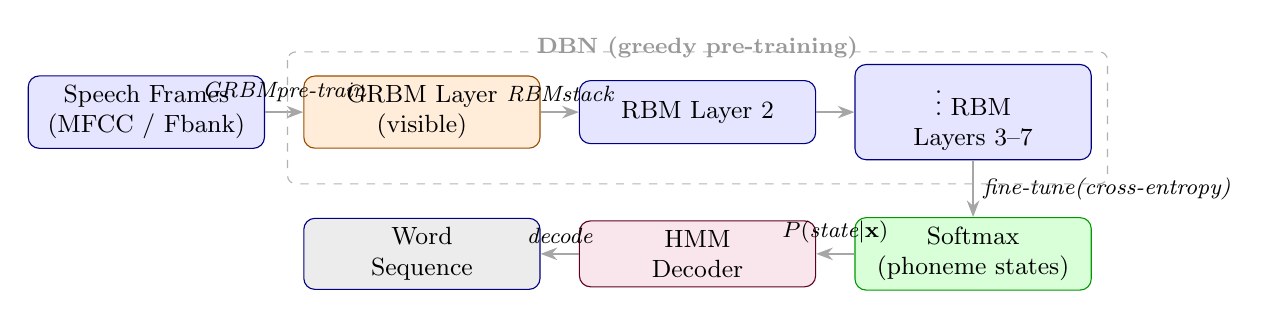
\begin{tikzpicture}[
  every node/.style={font=\small},
  block/.style={draw, rounded corners=4pt, minimum width=3.0cm, minimum height=0.8cm,
                align=center, fill=blue!10, draw=blue!50!black},
  arrow/.style={-{Stealth[length=6pt]}, thick, draw=gray!70},
  label/.style={font=\footnotesize\itshape}
]
\node[block] (feat) at (0,0) {Speech Frames\\(MFCC / Fbank)};
\node[block, fill=orange!15, draw=orange!60!black] (grbm) at (3.5,0) {GRBM Layer\\(visible)};
\node[block] (rbm1) at (7,0) {RBM Layer 2};
\node[block] (rbm2) at (10.5,0) {$\vdots$ RBM\\Layers 3--7};
\node[block, fill=green!15, draw=green!60!black] (softmax) at (10.5,-1.8) {Softmax\\(phoneme states)};
\node[block, fill=purple!10, draw=purple!50!black] (hmm) at (7,-1.8) {HMM\\Decoder};
\node[block, fill=gray!15] (words) at (3.5,-1.8) {Word\\Sequence};

\draw[arrow] (feat.east) -- node[above, label]{GRBM\\pre-train} (grbm.west);
\draw[arrow] (grbm.east) -- node[above, label]{RBM\\stack} (rbm1.west);
\draw[arrow] (rbm1.east) -- (rbm2.west);
\draw[arrow] (rbm2.south) -- node[right, label]{fine-tune\\(cross-entropy)} (softmax.north);
\draw[arrow] (softmax.west) -- node[above, label]{$P(\text{state}|\mathbf{x})$} (hmm.east);
\draw[arrow] (hmm.west) -- node[above, label]{decode} (words.east);

\draw[dashed, gray!60, rounded corners=3pt]
  ($(grbm.north west)+(-0.2,0.3)$) rectangle ($(rbm2.south east)+(0.2,-0.3)$);
\node[above, font=\footnotesize\bfseries, gray!80] at (7, 0.55) {DBN (greedy pre-training)};
\end{tikzpicture}
\caption{End-to-end pipeline for DBN-DNN acoustic modelling in ASR.
The DBN (dashed box) is pre-trained greedily layer-by-layer; the full system
is then fine-tuned discriminatively and integrated into an HMM decoder.}
\label{fig:asr-pipeline}
\end{figure}

\subsection{WER Comparison Results}

\cref{tab:wer-results} reproduces the landmark WER comparison table from the
lecture slides (Hinton et al., IEEE Signal Processing Magazine, Nov.\ 2012).

\begin{table}[ht]
\centering
\caption{Word Error Rate (\%) for various acoustic modelling techniques on the
HUB500-SWB and RT03S-FSH benchmarks (Hinton et al., 2012).
\#Params is in millions; NZ = non-zero parameters after sparsification.}
\label{tab:wer-results}
\begin{tabular}{lccc}
\toprule
\textbf{Modelling Technique} & \textbf{\#Params ($\times 10^6$)} &
\textbf{HUB500-SWB WER\%} & \textbf{RT03S-FSH WER\%} \\
\midrule
GMM, 40 mix DT 309H SI & 29.4 & 23.6 & 27.4 \\
NN 1 hidden layer $\times$ 4,634 units & 43.6 & 26.0 & 29.4 \\
+ 2$\times$5 neighbouring frames & 45.1 & 22.4 & 25.7 \\
\textbf{DBN-DNN 7 hidden $\times$ 2,048 units} & \textbf{45.1} & \textbf{17.1} & \textbf{19.6} \\
+ updated state alignment & 45.1 & 16.4 & 18.6 \\
+ sparsification & 15.2 (NZ) & 16.1 & 18.5 \\
\midrule
GMM 72 mix DT 2000H SA & 102.4 & 17.1 & 18.6 \\
\bottomrule
\end{tabular}
\end{table}

\begin{keyinsight}[title=The Speech Recognition Breakthrough]
  The DBN-DNN with 7 hidden layers $\times$ 2,048 units achieves \textbf{17.1\%}
  WER on HUB500-SWB -- a \textbf{6.5 percentage point} absolute improvement
  over the GMM baseline (23.6\%) and a staggering \textbf{8.9 point}
  improvement over a standard 1-hidden-layer NN (26.0\%).
  Four major research groups (Microsoft, Google, IBM, and the Hinton group)
  independently confirmed similar results around the same time, which gave the
  community high confidence that deep learning was a genuine breakthrough for
  speech recognition.
  For context, the speech recognition community had been struggling to reduce
  error rates below the 27\% range for nearly 30 years.
\end{keyinsight}

\subsection{Significance of the Speech Results}

Several aspects of \cref{tab:wer-results} deserve careful interpretation:

\begin{enumerate}[leftmargin=*, label=\arabic*.]
  \item \textbf{1-hidden-layer NN fails}: The single-hidden-layer NN (26.0\%)
        is actually \emph{worse} than the GMM (23.6\%), even with neighbouring
        frames.  This confirms that raw neural networks without proper
        initialisation cannot compete with well-tuned classical models.
  \item \textbf{Depth matters}: Adding more context frames (22.4\%) helps,
        but the 7-layer DBN-DNN (17.1\%) achieves a qualitatively different
        level of performance.
  \item \textbf{Comparable to a much larger GMM}: The DBN-DNN with 45.1M
        parameters matches the 102.4M-parameter GMM trained on \emph{six
        times more data} (2000 hours vs.\ 309 hours).  This is a dramatic
        demonstration of the data efficiency of deep representations.
  \item \textbf{Sparsification}: Pruning the network to 15.2M non-zero
        parameters (sparsification) barely degrades performance, indicating
        that the network has learnt a compact, distributed representation.
\end{enumerate}

\newpage

%% ===============================================================
\section{The Legacy of Greedy Pre-training and Modern Alternatives}
\label{sec:legacy}
%% ===============================================================

\subsection{Why Pre-training Is Less Necessary Today}

A student question in the lecture prompted Prof.\ Prasanna to address the
contemporary relevance of greedy pre-training.  Since 2012, several advances
have largely superseded the need for layer-wise pre-training when large amounts
of data are available:

\begin{enumerate}[leftmargin=*, label=(\roman*)]
  \item \textbf{ReLU activations}: The Rectified Linear Unit,
        $\sigma(z) = \max(0, z)$, has a gradient of 1 for positive inputs,
        which dramatically reduces the severity of the vanishing gradient
        problem compared to sigmoid/tanh.
  \item \textbf{Batch Normalisation}: Normalising layer inputs during
        training smooths the loss landscape, enabling reliable training of
        very deep networks from random initialisation.
  \item \textbf{Residual connections}: Skip connections in ResNets provide
        identity paths for gradients, allowing networks hundreds of layers
        deep to be trained directly.
  \item \textbf{Advanced optimisers}: Adam, RMSProp, and other adaptive
        learning-rate methods navigate the optimisation landscape more
        effectively than vanilla SGD.
  \item \textbf{Large datasets and transfer learning}: With millions of
        labelled training examples, models can be trained from scratch
        efficiently; and pre-trained models (e.g.\ BERT, GPT) provide
        powerful generic representations that can be fine-tuned.
\end{enumerate}

\begin{table}[ht]
\centering
\caption{Comparison of training regimes: greedy pre-training (2006) vs.\ modern
end-to-end training.}
\label{tab:modern-vs-pretrain}
\begin{tabular}{lcc}
\toprule
\textbf{Aspect} & \textbf{Greedy Pre-training (2006)} & \textbf{Modern End-to-end} \\
\midrule
Activation function & Sigmoid / tanh & ReLU / GELU \\
Weight initialisation & Layer-by-layer RBM/AE & Xavier / He initialisation \\
Normalisation & None & Batch norm, Layer norm \\
Gradient flow & Poor (vanishing) & Stable (residuals, ReLU) \\
Data requirement & Small to medium & Medium to large \\
Training complexity & High (two phases) & Single phase \\
Still useful? & Low-resource settings & General use \\
\bottomrule
\end{tabular}
\end{table}

\subsection{When Pre-training Still Matters}

As Prof.\ Prasanna explicitly noted: \emph{``if you have less amount of data,
for example you have a few hours of data and you want to train the deep
learning model, this greedy layer-wise training is still useful.''}

The modern analogue of greedy pre-training is \textbf{transfer learning} --
the practice of initialising a model with weights pre-trained on a large
dataset (e.g.\ ImageNet, Common Crawl) before fine-tuning on a target task.
This preserves the spirit of the 2006 insight: starting in a good region of
weight space reduces the burden on the final discriminative fine-tuning step.

\begin{keyinsight}[title=The Enduring Principle]
  The fundamental insight of Hinton and Bengio (2006) was not merely an
  engineering trick: it demonstrated that \emph{good weight initialisation
  matters enormously} for deep network training.  Modern techniques
  (He initialisation, batch normalisation, residual connections) achieve the
  same goal -- placing the initial weights in a region where gradient flow is
  healthy -- by different means.  Greedy pre-training solved the right
  problem; later advances solved it more efficiently.
\end{keyinsight}

\subsection{Connection to Modern Self-supervised Learning}

There is a deep conceptual connection between 2006-era greedy unsupervised
pre-training and modern self-supervised learning methods:

\begin{itemize}[leftmargin=*]
  \item \textbf{BERT} (Devlin et al., 2019) pre-trains a Transformer by
        masking and reconstructing tokens -- a form of auto-encoding at the
        sequence level.
  \item \textbf{Contrastive learning} (SimCLR, MoCo) pre-trains visual
        encoders by learning representations invariant to augmentations.
  \item \textbf{wav2vec~2.0} pre-trains speech encoders by discretising and
        reconstructing speech features -- directly analogous to the acoustic
        modelling pipeline in \cref{sec:asr}.
\end{itemize}

In all these cases, unsupervised/self-supervised pre-training provides a
better initialisation than random weights, and the model is then fine-tuned
discriminatively -- precisely the two-phase strategy of Hinton et al.\ (2006).

\newpage

%% ===============================================================
\section{Session Summary and Conclusions}
\label{sec:summary}
%% ===============================================================

Session~10 presented the theoretical foundations and landmark empirical
evidence for the 2006 breakthrough in deep learning.  The following key
points summarise the session:

\begin{enumerate}[leftmargin=*, label=\textbf{\arabic*.}]
  \item \textbf{The problem}: Deep networks trained from random initialisation
        suffered from vanishing/exploding gradients, performing no better --
        and often worse -- than shallow networks or SVMs (e.g.\ 2.95\% MNIST
        error vs.\ 1.4\% SVM).

  \item \textbf{The insight}: The greedy layer-wise algorithm, previously used
        in the \emph{feedback} (RBM) network literature, could be repurposed
        for initialising \emph{feedforward} deep networks.

  \item \textbf{The unsupervised variant} (Hinton et al., 2006): Pre-train
        each layer as a GRBM/RBM using reconstruction error as the objective.
        Stack the pre-trained layers to form a Deep Belief Network (DBN), then
        fine-tune end-to-end.  Result: \textbf{1.25\%} MNIST error (vs.\
        1.4\% SVM).

  \item \textbf{The supervised variant} (Bengio et al., 2006, NIPS): Pre-train
        each layer as a 1-hidden-layer auto-encoder with the input as its own
        target.  Discard the decoder.  Fine-tune end-to-end.  Result:
        comparable to SVM; weaker than unsupervised, but proved the concept.

  \item \textbf{Speech recognition breakthrough}: Four major groups
        (Microsoft, Google, IBM, Hinton) independently demonstrated that
        DBN-DNN acoustic models reduced WER from 23.6\% to 17.1\% on
        HUB500-SWB -- a 6.5 point absolute improvement after decades of
        stagnation around 27\%.

  \item \textbf{Historical significance}: These two papers -- Hinton (2006)
        and Bengio (2006) -- are the cornerstone papers of the modern deep
        learning era.  They provided the algorithmic proof-of-concept that
        directly motivated the investment and research that produced AlexNet
        (2012), Transformers (2017), and large language models.

  \item \textbf{Modern relevance}: Greedy pre-training is no longer the
        standard method for large-data regimes, superseded by ReLU, batch
        normalisation, residual connections, and Adam.  However, for
        low-resource settings, its principles remain valid and are echoed
        in modern self-supervised and transfer learning approaches.
\end{enumerate}

\begin{example}[Timeline of Breakthroughs Covered in Sessions 1--10]
  \begin{center}
  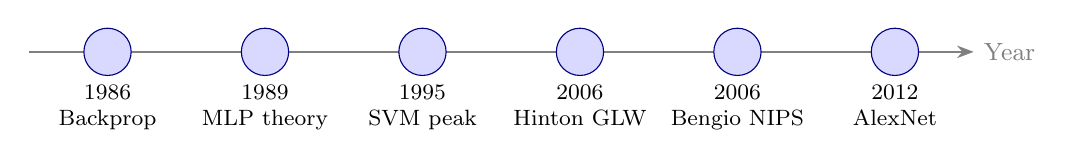
\begin{tikzpicture}[
    every node/.style={font=\small},
    event/.style={circle, draw=blue!50!black, fill=blue!15, minimum size=0.6cm},
    timeline/.style={-{Stealth[length=6pt]}, thick, gray}
  ]
  \draw[timeline] (0,0) -- (12,0) node[right]{Year};
  \foreach \x/\yr/\lab in {
    1/1986/Backprop,
    3/1989/MLP theory,
    5/1995/SVM peak,
    7/2006/Hinton GLW,
    9/2006/Bengio NIPS,
    11/2012/AlexNet/DNN ASR
  }{
    \node[event] at (\x,0) {};
    \node[below=0.3cm, align=center, font=\footnotesize] at (\x,0) {\yr\\\lab};
  }
  \end{tikzpicture}
  \end{center}
\end{example}

\subsection{Take-away Messages}

\begin{itemize}[leftmargin=*]
  \item \textbf{Conceptual}: A good initialisation is as important as the
        architecture.  Greedy pre-training solved initialisation; modern
        techniques (He init, BN, residuals) solve it differently.
  \item \textbf{Practical}: When data is scarce, consider layer-wise
        pre-training or transfer learning before end-to-end training.
  \item \textbf{Historical}: Read the Hinton 2006 and Bengio 2006 papers.
        As Prof.\ Prasanna noted, ``there is no mathematical equation
        there'' -- great ideas are often elegant and simple.
  \item \textbf{Forward-looking}: The self-supervised learning paradigm
        (BERT, wav2vec, CLIP) is the modern embodiment of the same core
        principle: pre-train on reconstruction/contrastive objectives, then
        fine-tune discriminatively.
\end{itemize}

\newpage

%% ===============================================================
\section*{References}
\addcontentsline{toc}{section}{References}
%% ===============================================================

\begin{enumerate}[leftmargin=*, label={[\arabic*]}]

  \item G.\ E.\ Hinton, S.\ Osindero, and Y.-W.\ Teh, ``A fast learning
        algorithm for deep belief nets,'' \textit{Neural Computation},
        vol.\ 18, no.\ 7, pp.\ 1527--1554, 2006.

  \item Y.\ Bengio, P.\ Lamblin, D.\ Popovici, and H.\ Larochelle,
        ``Greedy layer-wise training of deep networks,''
        \textit{Advances in Neural Information Processing Systems (NIPS)},
        vol.\ 19, 2006.

  \item G.\ E.\ Hinton, L.\ Deng, D.\ Yu, G.\ Dahl, A.\ Mohamed,
        N.\ Jaitly, A.\ Senior, V.\ Vanhoucke, P.\ Nguyen, T.\ N.\ Sainath,
        and B.\ Kingsbury,
        ``Deep neural networks for acoustic modeling in speech recognition,''
        \textit{IEEE Signal Processing Magazine}, vol.\ 29, no.\ 6,
        pp.\ 82--97, Nov.\ 2012.

  \item G.\ Tesauro, ``Practical issues in temporal difference learning,''
        \textit{Machine Learning}, vol.\ 8, no.\ 3--4, pp.\ 257--277, 1992.

  \item I.\ Goodfellow, Y.\ Bengio, and A.\ Courville,
        \textit{Deep Learning}. MIT Press, 2016.
        \url{https://www.deeplearningbook.org}

  \item Y.\ LeCun, L.\ Bottou, Y.\ Bengio, and P.\ Haffner,
        ``Gradient-based learning applied to document recognition,''
        \textit{Proceedings of the IEEE}, vol.\ 86, no.\ 11,
        pp.\ 2278--2324, 1998.

  \item J.\ Devlin, M.-W.\ Chang, K.\ Lee, and K.\ Toutanova,
        ``BERT: Pre-training of deep bidirectional transformers for
        language understanding,'' \textit{NAACL-HLT}, 2019.

\end{enumerate}

\vspace{2em}
\hrule
\vspace{0.5em}
\noindent\small\textit{These notes were compiled from the lecture transcript
and visual extractions of Session~10 (Video: \url{https://vimeo.com/1148825885};
Slides: \url{https://learning.iiitdwd.ac.in/mod/resource/view.php?id=1352}).
Department of Data Science and Artificial Intelligence,
Indian Institute of Information Technology Dharwad.}

\clearpage

\end{document}
